
%%\documentclass{article}
\documentclass{scrartcl}

\usepackage{cmap}
\usepackage{booktabs}
\usepackage{colortbl}
\usepackage{multirow}
\usepackage{subfloat}
\usepackage{float}
\floatstyle{boxed} 
\restylefloat{figure}

\usepackage{lipsum}

\usepackage{kpfonts}

\usepackage{polyglossia}
\setdefaultlanguage{english}

%\usepackage[backend=biber]{biblatex}
\usepackage[backend=biber, style=ieee]{biblatex}
\addbibresource{beauty.bib}

\usepackage{graphicx}
\graphicspath{ {./photos/} }






\begin{document}

\begin{titlepage}


\title{\textsc{\LARGE Bern University of Applied Sciences | BFH }\\[1cm]
\begin{center}

\includegraphics[width = 60mm]{bea_logo.JPG}
\end{center}
\textsc{\small Department of Engineering and Information Technology}\\
\textsc{\small Project2 (Module BTI7302) 19/20}\\[1cm]
\textsc{\small Report on management system for: }\\
\textsc{"Academy of the handsome men and beautiful woman(BEA)" web application}}
\date{\today}   %% or \date{01 november 2019}
\author{\textit{author: }Kristina \textsc{Shiryagina} (\texttt{kristina.shiryagina@bfh.ch}) \\
 \textit{supervisor: } Prof.Dr Olivier  \textsc{Biberstein}  (\texttt{olivier.biberstein@bfh.ch})\\
 }
\maketitle	
	
\tableofcontents
\clearpage
\end{titlepage}


\section{Abstract}
/**The abstract may not be what you write first, as it might be easiest to summarize your whole paper after it's been completed. You could draft it from your outline, but you'll want to double-check later that you have included the most important points from your article and that there's nothing in the abstract that you decided not to include in your report.., max 250 words*/\\

The purpose of this research was to produce a  part of E-learning management system that could provide everything needed for a partially automated  E-learning system. Using the scrum developing process, I have divided the development into five phases. Those were analysis, the architecture of the application, design, implementation, testing. Analysis phase was done by finding user stories, making domain model and different analyses. The architecture of the application was done by deciding what I will use for the architecture of this application, by researching modern technologies. The designing phase used Unified Modelling Language (UML), and the implementation phase used Java language with Spring Boot framework for backend, Angular Framework with TypeScript , html, css, for frontend. Then, testing used different tests and questionnaire as a user acceptance test. In the end, this research could produce a Part of Learning Management System (LMS) namely Online Learning System. It can help participants do different courses, to find learning materials for the course they want to do, monitor, and assess their learning progress through the quiz, order an online exam with a teacher, see his evaluation. It can be very useful for lecturers to make online tutorials, to upload different learning files, to make online exams. And it can be very useful for administrators, who manage different information on this online education application.

 



\section{Main steps of this work}


\subsection{Introduction and Vision of this project}
  \subsubsection{What is it E-learning and why it is so popular}
  	
This project is a component of E-learning system. \\
E-learning is education via the Internet, network, or standalone computer. E-learning is basically the network-enabled convey of skills and knowledge. E-learning refers to using electronic applications and processes to learn. It includes all forms of electronically supported learning and teaching.\\
 E-learning is the computer and network-enabled transfer of skills and knowledge. E-learning applications and processes include Web-based learning, computer-based learning, virtual education opportunities and digital collaboration.\\
E-learning systems contain both Learning Management System and Course management system. It can be self-paced or instructor-led and includes media in the form of text, image, animation, streaming video and audio. It is commonly thought that new technologies can make a big difference in education.
Efficient acquisition, storage, transfer, retrieval, application, and visualization of knowledge often distinguish successful organizations from the unsuccessful ones. The ability to obtain, assimilate, and apply the right knowledge effectively will become a key skill in this century. Learning is the key to achieving our full potential.\\
With the rapid change in all types of working environments, there is a constant need to rapidly train and retrain people in new technologies, products, and services found within the environment.\\
\subsubsection{Future system}

As the head of information system for Online academy, I have tasked with developing a part of a new Online Management System for E-learning. As the idea of online education is getting more popular day by day. \\
The proposed software product (Online Beauty academy) is an online education system. The system will be used for online education, to study online-courses, to view and download different lectures, conducting online quizzes, course registration, exam reservation, managing results. The system must be right protected.\\
This product let persons who have the interest to study beauty, who want to make them self more beautiful to do it. It will offer also other different online courses. 
 Each course will have topics and lessons for each topic. The context of lessons are text, video tutorials, etc. \\
 There is a possibility to get a certificate by passing corresponding exams of each course.


Online Exams.\\
 This application will establish a network between the lecturers and participants. Academia enters the questions they want in the exam. These questions are displayed as a test for the eligible participant. The answers entered by the participant are then evaluated and their score is calculated and saved. This score then can be accessed by the Academy to evaluate the performance of participants.
Exam details.\\
Each topic will have a small exam(quizzes). Making exams the participant will collect points. The sum of all point for all small exams is 30\% of the final grade. After making all small exams participant will be able to make a final exam that has weight 70\% of the final grade. The participant must make a reservation for the final interactive exam with lecturers. He has to choose the available Date for this exam. ´\\

The application has an administrator who keeps an eye on the overall functioning of the system.

  	
  	\subsubsection{Problem Statement}
  	Now academies are running various programs as full-time courses. The academy timing sometimes makes it difficult to study for the persons who are doing some jobs. The online education would help such persons who live far away from educational institutes.
The other problem is that the current online management system doesn't have the needed flexibility and is not modern enough. The capabilities are limited.
An online management system is effective, reduce time and cost in courses and exam management process.

  	\subsubsection{Stakeholder Summary}
  	Similar to other technology applications, the success of online-learning is dependent on the extent to which it satisfies the needs and addresses the concerns of its stakeholders.
  	\begin{itemize}
  	\item Participant: use the system to register for the course or exam, view 			information.
  	\item Instructors: they could give ideas on the solution for the system’s development and improvement.
  	\item Administrator: manage the system after it is built.
  	\item Education Institutions 
  	\item Content Providers
  	\item Development team: include all software engineers, business analysts, system analysts, system designers, implementer, testers, QA, and project management. They are tasked to build the system.
  	\item Employers
  	\end{itemize}
  	
  	\subsubsection{Objective of the project}
  	The main goal of this project is to make part of this big system. It will include use cases for the user, participant, lecturer and administrator. 
  Now I want to describe the main goals that I have planned to do during this semester. \\The first goal is to make the user possible to register himself in this application. The system has to be able to recognize the different roles of the user. The system has to be well secured, for this purpose. I will use the security staffs that offers spring boot framework. Then user can easily login in the system and see all available courses in the course catalogue. \\
  For the administrator it is necessary to implement managing tools, so that administrator can manipulate courses, like add a new course, delete, update, etc. I will implement also the administrator tools to manipulate all users.\\
  The other goal is to make it possible user to register for the course that he likes. And one more goal is to make it possible participant to order an exam. 
  
  
  	\subsubsection{Product Overview}
  
  	This section provides a high-level overview of the BEA(Beautiful academy) features for various types of roles.
 The user can list courses. 
 Our user can easily register his self for courses he likes and follows the program of this course. Each course has topics and lessons for each topic. The context of lessons are text, video tutorials, etc. \\
  	The user can test himself with mini exams. The user can also choose a final exam with the lecturer. Our academy gives the possibility to have a certificate. For this, the user has to make all required exams for the course and if he passed es well he will become a certificate from our academy. \\
  	This application is also very useful for lecturers. The lecturer can use this system to upload content of courses, topics, lessons. The lecturer can make online tutorials for participants. He can give online exams. He can make an evaluation. He can prepare the content of quizzes needed for mini exams.\\
  	The administrator can create, change, delete, update and control information about courses, lectures, users, date and time, etc.
  	
  	
  	\subsubsection{Summary of System Features}
  	
  	\begin{itemize}
  	\item Online registration.
  	\item Log in.
  	\item Manage User information.
  	\item Manage Offering Courses.
  	\item Course registration.
  	\item Exam registration (order an exam).
  	\end{itemize}
  	
  	\subsubsection{Summary of Future Features}
  	\begin{itemize}
  	\item Manage Financial Activities.
  	\item Uploading course content.
  	\item Course evaluation.
  	\item Downloading course content.
  	\item Video conferencing.
  	\item Info service.
  	\item Information library.
  	\end{itemize}
  	
  	
  	\subsubsection{Use Cases }
  	For level access control, users are divided into four levels of access, namely , user, participant, lecturer and administrator. This levels of access have different access control to BEA  as seen in use case diagrams in Figure 1  and Figure 2
  	\begin{figure}[H]
\centering
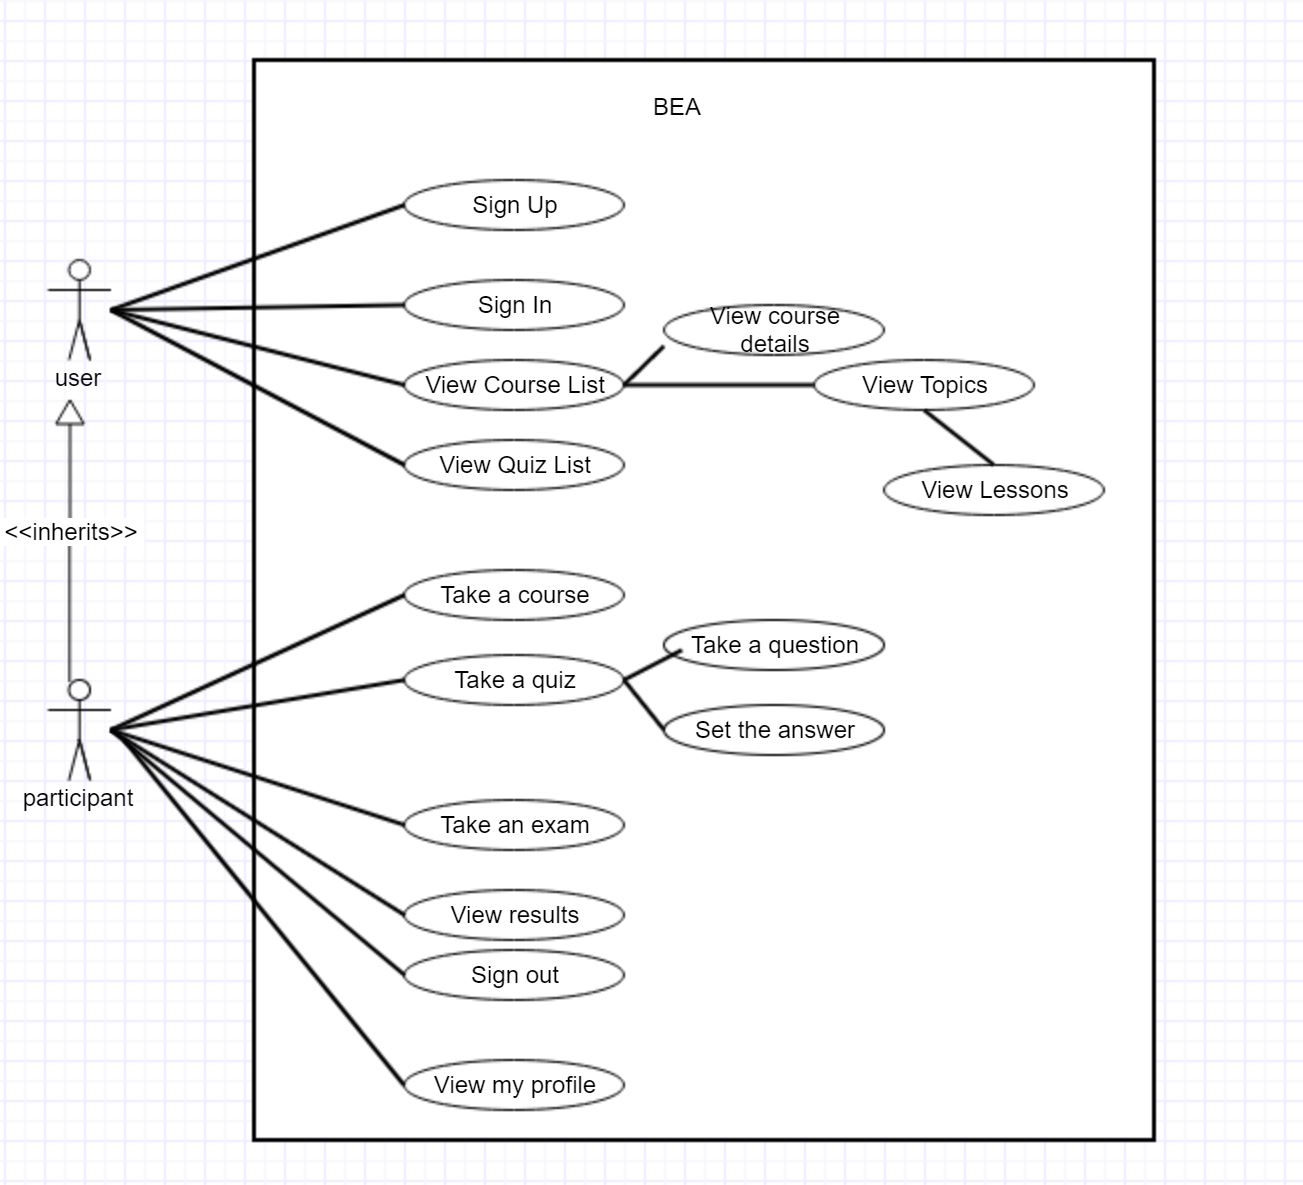
\includegraphics[width=150mm]{ucd_user.JPG}
\caption{Use Case Diagram for user of BEA}
\label{ucd_user}
\end{figure}

\begin{figure}[H]
\centering
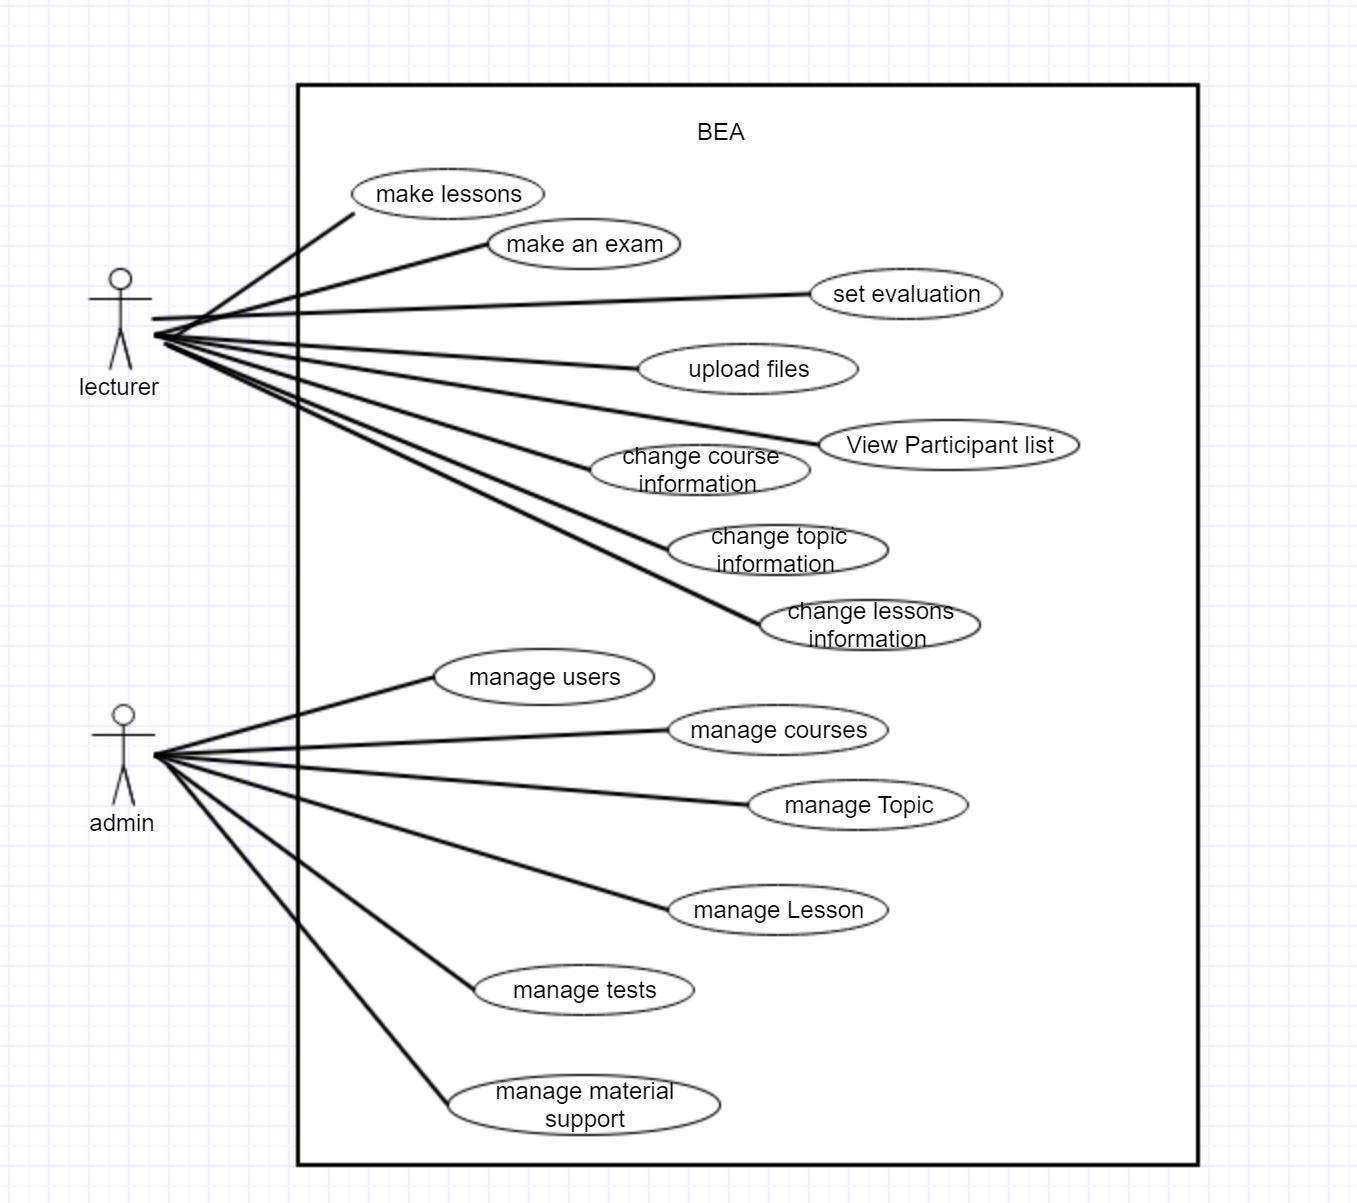
\includegraphics[width=150mm]{ucd_admin_lecturer.JPG}
\caption{Use Case Diagram for administrator and lecturer of BEA}
\label{ucd_user}
\end{figure}

  	\subsection{Software development methodology}
  	The establishment and use of sound engineering principles in order to obtain economically
developed software that is reliable and works efficiently on real machines is called software engineering.\\
\textbf{\textit{ Software engineering}} is the discipline whose aim is:\\
1. production of quality software\\
2. software that is delivered on time\\
3. cost within the budget\\
4. satisfies all requirements.\\
\textbf{\textit{ Software process}} is the way in which we produce the software. Apart from hiring smart,
knowledgeable engineers and buying the latest development tools, effective software
development process is also needed, so that engineers can systematically use the best technical
and managerial practices to successfully complete their projects.\\
A \textbf{\textit{ Software life cycle}} is the series of identifiable stages that a software product undergoes during
its lifetime. A software life cycle model is a descriptive and diagrammatic representation of the
software life cycle. A life cycle model represents all the activities required to make a software
product transit through its life cycle phases. It also captures the order in which these activities are
to be taken .\\



\subsubsection{ Agile development, Scrum.} 
Scrum was in the centre of the developing process.
As scrum projects make progress in a series of “sprints”, we have divided the whole process into
4 sprints. Product was first analysed, designed, then code and tested during the sprint. \\
Scrum
Roles \\
	•	Scrum Master – Prof.Dr. Olivier Biberstein\\
	•	Developer – Kristina Shiryagina\\
 Artifacts \\
	•	Product Backlog\\
	•	Sprint Backlog\\
 Meetings have included :\\
	•	Product/release planning\\
	•	Sprint planning\\
	•	Weekly Scrum\\
	•	Sprint review\\
	•	Sprint retrospective\\
Scrum Meetings \\
Each meeting between developer and scrum master was made of several steps, that were repeated each time:\\
	•	Attendance: all\\
	•	Product Owner presents Product Backlog\\
with all relevant user stories with their priority\\
	•	Discussions and clarifications if needed\\
	•	Results:\\
Prioritized Product Backlog\\
	•	Specifies what to build\\
	•	A final decision by the Master\\
	•	Vision, high-level architecture, most important non-functional\\
requirements\\
Release planning (if the product is to be delivered in releases):\\
	•	Select and prioritize items of Product Backlog for the next Release Backlog \cite{sed}\\
	
	

\begin{table}[h]
\begin{center}
\begin{tabular}{| p{7cm}| p{7cm} |}
Our developments steps \\
\hline
\textbf{Phase} & \textbf{Processes} \\
\hline
Initiate                    &             In this phase I've created project vision, priories Product Backlog and conduct release planning \\ \hline
Analysis                    &             Functionalities (user stories, use cases), Domain model. In this phase I have made different analyses, First I've made User stories, then I have found the concept classes and made a domain model.\\ \hline
Architecture of the application                   &           \\ \hline
Design                   &        In this phase I've created  System sequence diagrams, Sequence diagrams, Design class diagrams. These diagrams are very important to make implementation. \\ \hline
Implementation                   &           For Implementation I have chosen the Spring Framework for backend and Angular Framework for frontend.\\ \hline
Testing                   &            For test this application I have used: Unit test and other tests that I describe later\\ \hline

\end{tabular}
\end{center}
\caption{Caption2}
\label{table2}
\end{table}

\subsection{Feasibility}
\subsubsection{Technical Feasibility}
This project is a web-based application. The main technologies and tools:
\begin{itemize}
  	\item HTML
  	\item CSS
  	\item TYPESCRIPT 3.5.3
  	\item FREE MAKER(ftl)
  	\item Java 1.8
  	\item SPRING-BOOT 
  	\item @angular/cli  8.3.20
  	\item @angular/material  7.3.7
  	\item PostgreSQL  11.2
  	\item INTELIJ IDEA  2018.3.5
  	\item GIT  2.20.1.windows.1
  	\item GIFFY(DIAGRAM DRAWING TOOL)
  	\item LATEX 3.14159265-2.6-0.99999 (TeX Live 2019/dev/Debian)

  
  	
  	\end{itemize}
 \subsubsection{Financial Feasibility}
 Being a web application BEA will have a hosting cost.
 \subsubsection{Resource and Time Feasibility}
 \begin{itemize}
 \item Laptop (programming device)
 \item Hosting
 \item Programming tools
 \end{itemize}
 


\subsection{Analysis} 	 
\subsubsection{Domain model}  
\begin{figure}[h]
\centering
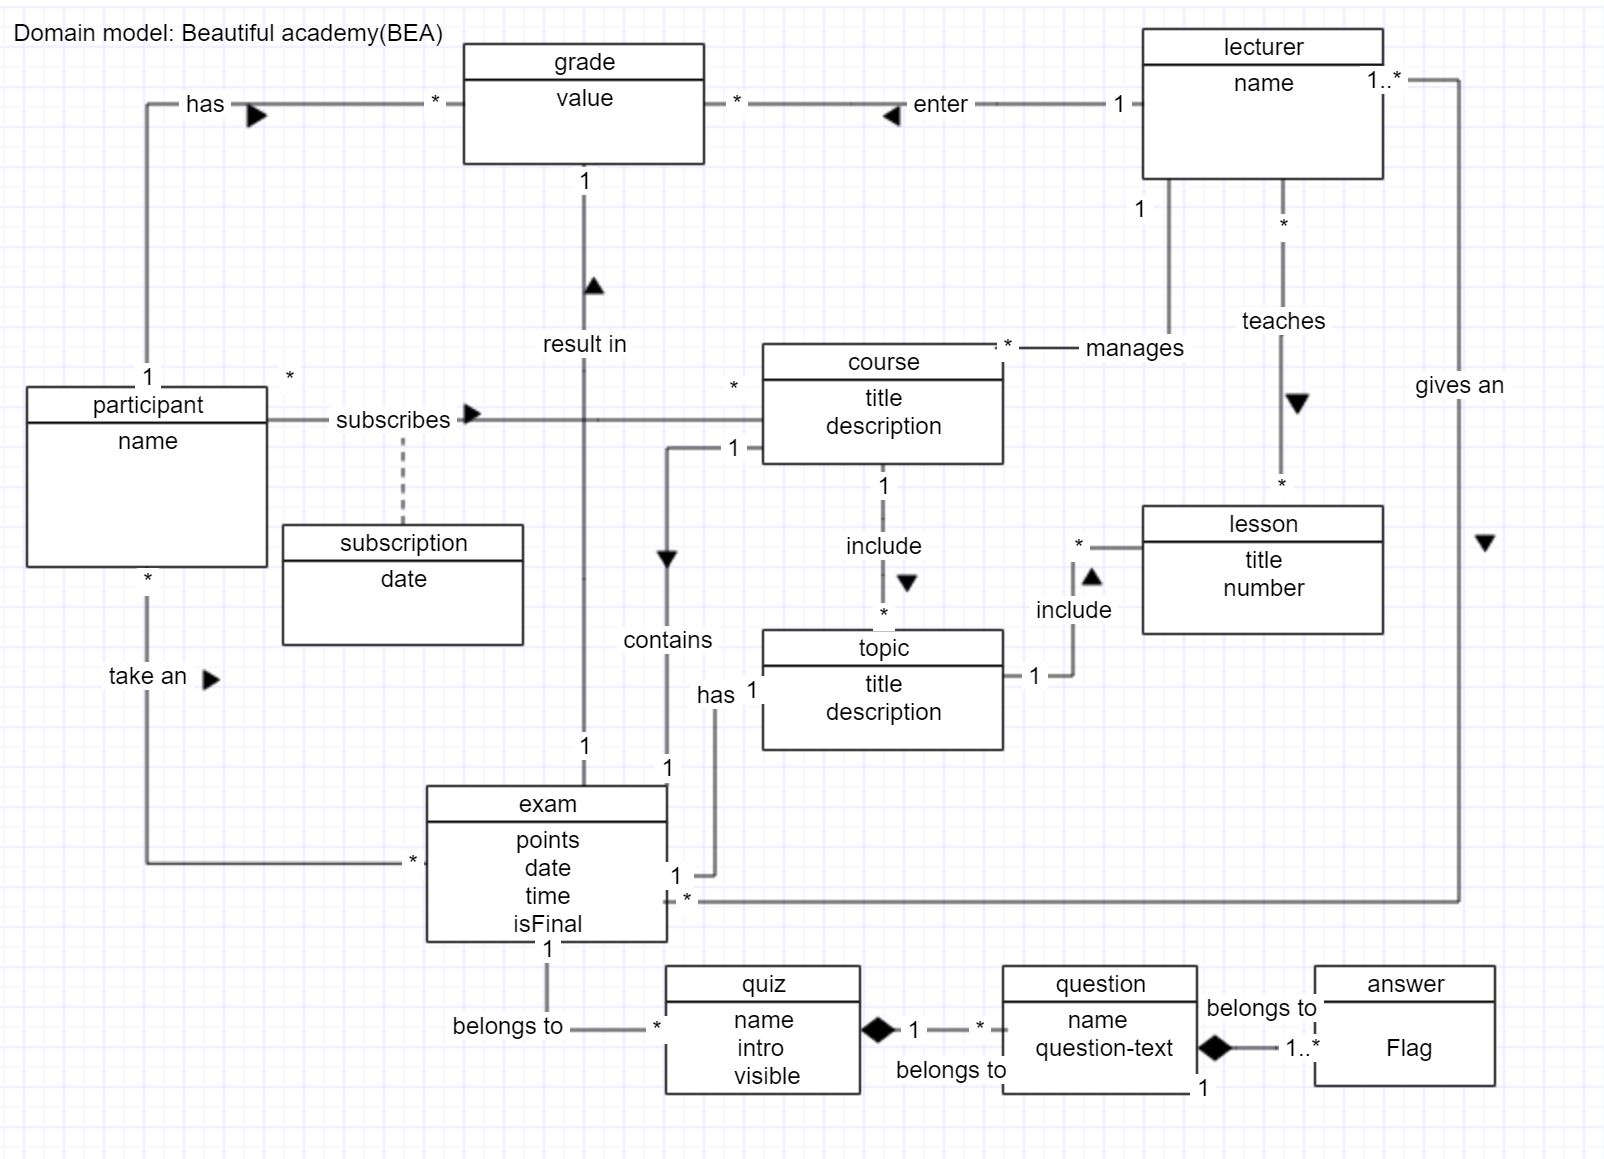
\includegraphics[width=150mm]{domain-in-use.JPG}
\caption{This is a Domain model for Beautiful academy(BEA)}
\label{Life Cycle Models}
\end{figure}

This document describes the domain model of the Beautiful Academy BEA. It introduces the most important concepts and the associations among them. It also introduces the respective multiplicities. \\

Concept Classes \\

Concept class Participant models a person who is taking the courses. \\
Concept class Lecturer models a person who is teaching and give an exam for the participant.\\
Concept class Course models the main courses that offer application.\\
Concept class Grade models the grades of a participant.\\
Concept class Topic models the sub course of the course.\\
Concept class Lesson models a set of lessons that contain each topic.\\
Concept class Exam models an exam that can be taken by the participant.\\
Concept class Subscription models a subscription, that has a date when the participant is subscribed.\\
Concept class Quiz models a quiz that belongs to the exam.\\
Concept class Question models a question that belongs to a quiz.\\
Concept class Answer models a possible answer to questions.\\

Associations\\

Association take an between Participant and Exam denotes the fact that Participant can make many exams, hence (*) multiplicity, and (*) multiplicity at the Exam side means that the  Exam can be done by many Participants.\\
Association has between Participant and Evaluation denotes the fact that Participant can get zero or more Evaluations, hence multiplicity (0..*), and (1 )multiplicity at the Participant side means that each Participant has its own set of Evaluation.\\
Association subscribes between Participant and Course denotes the fact that that zero or more Participant can be entered to the Course depending of the number of participants, hence multiplicity(*), and each Participant can be subscribed to zero more courses, hence multiplicity(*)\\
Association result in between Exam and Evaluation denotes the fact that each exam has its own unique evaluation, hence multiplicity 1, and 1 multiplicity at the evaluation side means that each evaluation belongs to the unique exam.\\
Association has between Exam and Topic denotes the fact that each topic has it’s unique an intermediate exam. \\
Association contains between Exam and Course denotes the fact that each exam belongs to its unique course, and each course has its own unique final exam. \\
Association include between Course and Topic denotes the fact that course has many topics, hence multiplicity (*), and each topic belongs to exactly one course, hence multiplicity (*). \\
Association include between Topic and Lesson denotes the fact that topic has many lessons, hence multiplicity (*), and each lesson belongs to exactly one topic, hence multiplicity (*). \\
Association teaches between Lecturer and Lesson denote the fact that Lecturer can teaches zero or more lessons, hence multiplicity (*), and each lesson can have zero or more lecturer, hence multiplicity (*). \\
Association gives an between Lecturer and Exam denotes the fact that Lecturer can give zero or more exam, hence multiplicity (*), and each exam can be done by 1 or more lecturer, hence multiplicity ( 1..*). \\
Association enter between the Lecturer and Evaluation denotes the fact that each lecturer can enter zero or more evaluations, hence multiplicity (*), and evaluation can be entered by exactly one lecturer, hence multiplicity (1). \\
Association manages between the Lecturer and Course denotes the fact that each lecturer can manage zero or more courses, hence multiplicity (*), and each course can be managed by exactly one lecturer, hence multiplicity (1). \\
Association belongs to between Quiz and Exam denotes the fact that each Quiz belongs to exactly one exam, hence multiplicity (1), and each exam can have zero or more quizzes, hence multiplicity(0..*). \\
Association belongs to between Quiz and Question denotes the fact that each Question belongs to exactly one Quiz, hence multiplicity (1), and each Quiz can have zero or more questions, hence multiplicity(0..*). \\
Association belongs to between Question and Answers denotes the fact that each Answer belongs to exactly one Question, hence multiplicity (1), and each exam can have one or more answer, hence multiplicity(1..*). \cite{sed}\\
\subsubsection{Product Backlog and user stories}
The product backlog is a list of user stories which is used to implement the product vision. It is sorted according to the priority of the user stories according to the product owner. The priority of these stories will be modified during the process of the project.\\


 

  \begin{table}[H]
\begin{center}
\textbf{USER STORIES }\\[1cm]
\begin{tabular}{| p{2.5cm}| p{4cm} | p{9cm} |}
\hline
\textbf{id} & \textbf{Story name} & \textbf{Story description}\\
\hline      
	
	1.0 & Login & As a user, I want to be able to login into the system with my credential (username, password).
 Success: The user is logged in and can use the functionality of the system.
 Failure: An error message is displayed: “Wrong username or password, please try again!”. \\ \hline
	2.0 & List courses & As a Participant, I want to list courses I'm entitled to subscribe such that I can perform a subscription. \\ \hline
	3.0 & View information & As a Participant, I want to see the information about the courses. \\ \hline
	4.0 & List results & As a Participant, I want to see my marks of the already finished courses and topics. \\ \hline
	5.0 & View schedule & As a Participant or a Lecturer, I want to be able to get a schedule showing the time and place of available exams. \\ \hline
	6.0 & Exam reservation & As a Participant, I want to be able to select an exam (there are different data on an exam).
 Success: A participant has selected exam.
 Failure: An error message is displayed “This date is already reserved, please take another date for your final exam". \\ \hline
	7.0 & Cancellation of exam & As a Participant, I want to be able to cancel the exam registration.
 Success: A message “You have successfully deleted your exam registration”
 Failure: An error message "The period of availability of deleting registration is expired, please take a contact to the administration". \\ \hline
	8.0 & Personal information & As a Participant or a lecturer I want to see my page with my personal information.
 Success: The participant can see his page with all the information it has.
 Failure: We are sorry, this page is on reconstruction, you can access it after 12 hours. \\ \hline
	9.0 & Manage course & As a System Administrator, I want to be able to change the information on a course.
 
 \\ \hline
	10.0 & List participants and corresponding courses & As a lecturer, I want to see a list of participants with courses that they have.
 
\\ \hline


        
        \end{tabular}
\end{center}
\caption{Product Backlog}
\label{table2}
\end{table}

\subsection{Design}
\subsubsection{System Sequence Diagrams}
 Use case "Log in"
\begin{figure}[H]
\centering
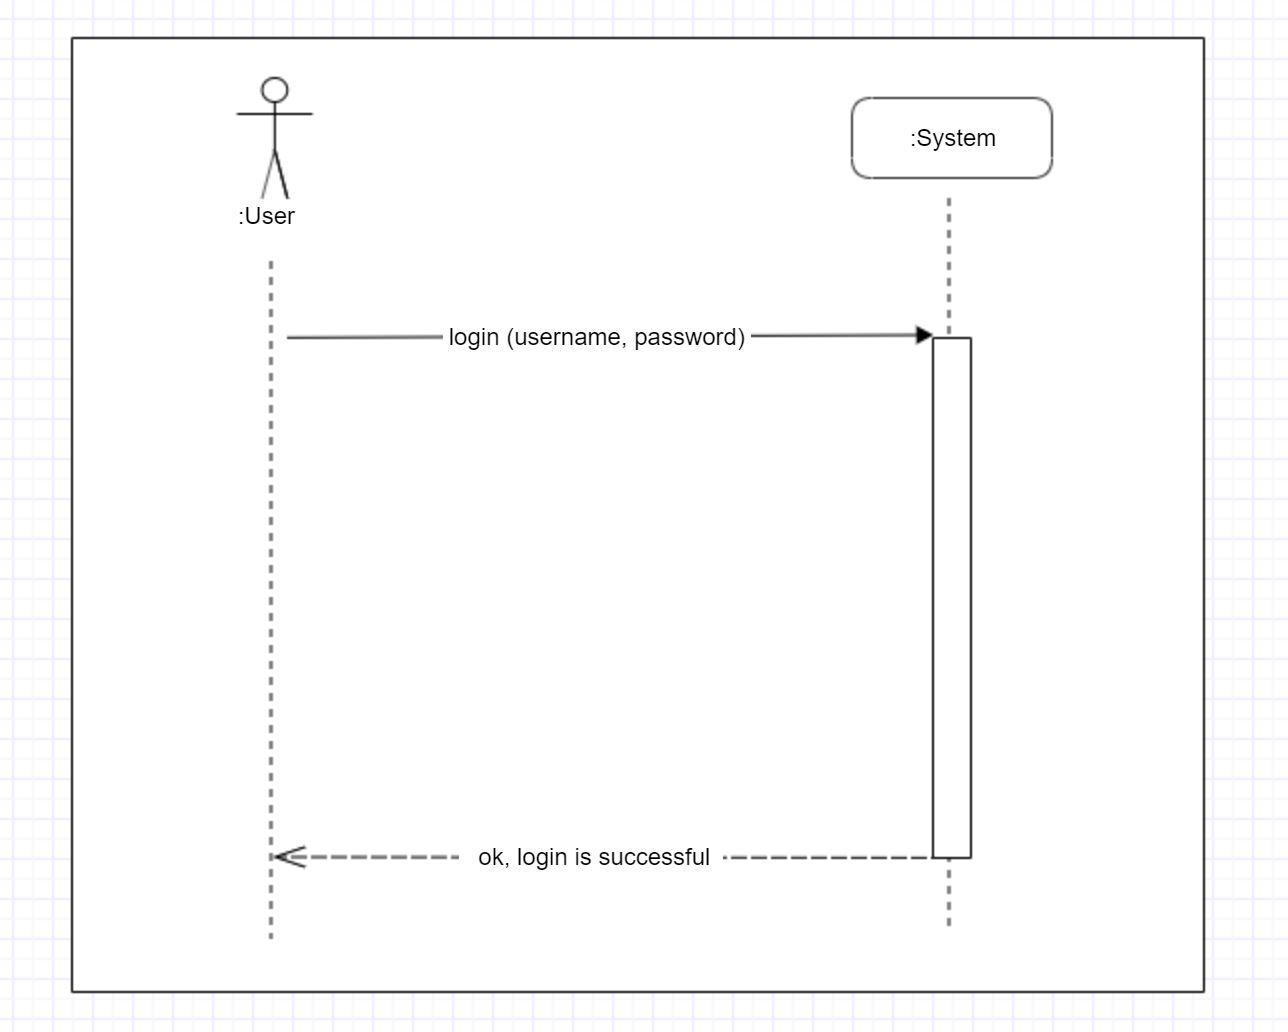
\includegraphics[width = 100mm]{ssd-login.JPG}
\caption{ssd for login}
\label{ssd for login}
\end{figure}


Use case "Registration"
\begin{figure}[H]
\centering
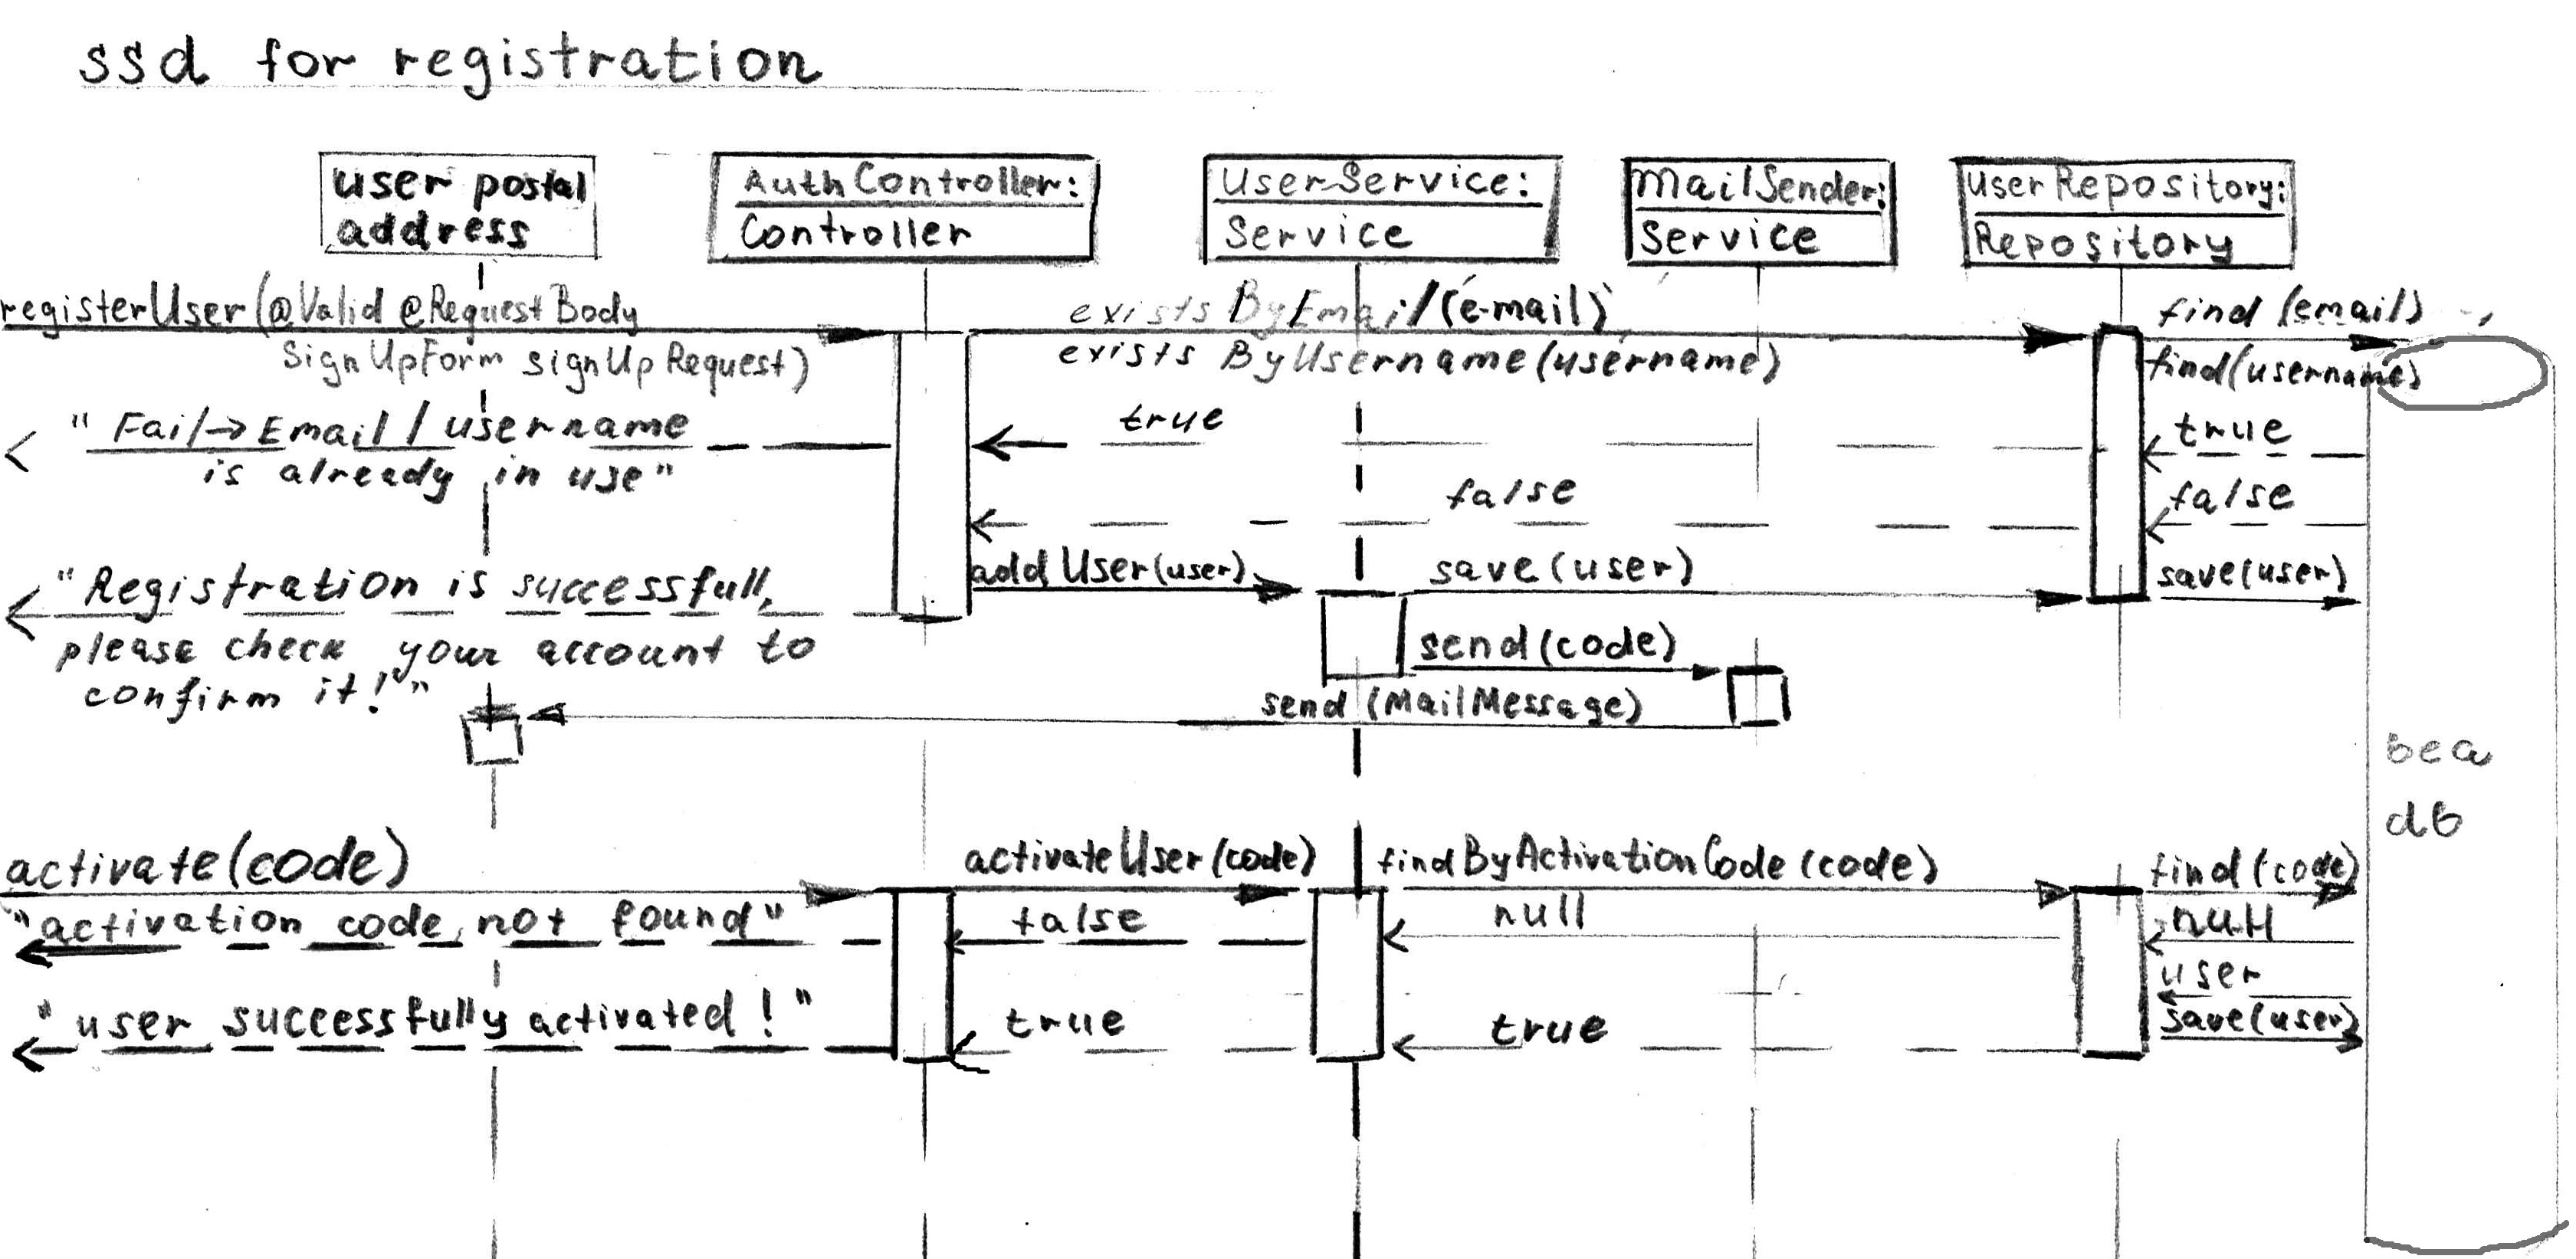
\includegraphics[width = 140mm]{ssd-reg.JPG}
\caption{ssd for registration}
\label{ssd for registration}
\end{figure}

\newpage
%sd for course managing 
Use case "Manage offering Courses"\\
\textbf{Create a course}
\begin{figure}[H]
\centering
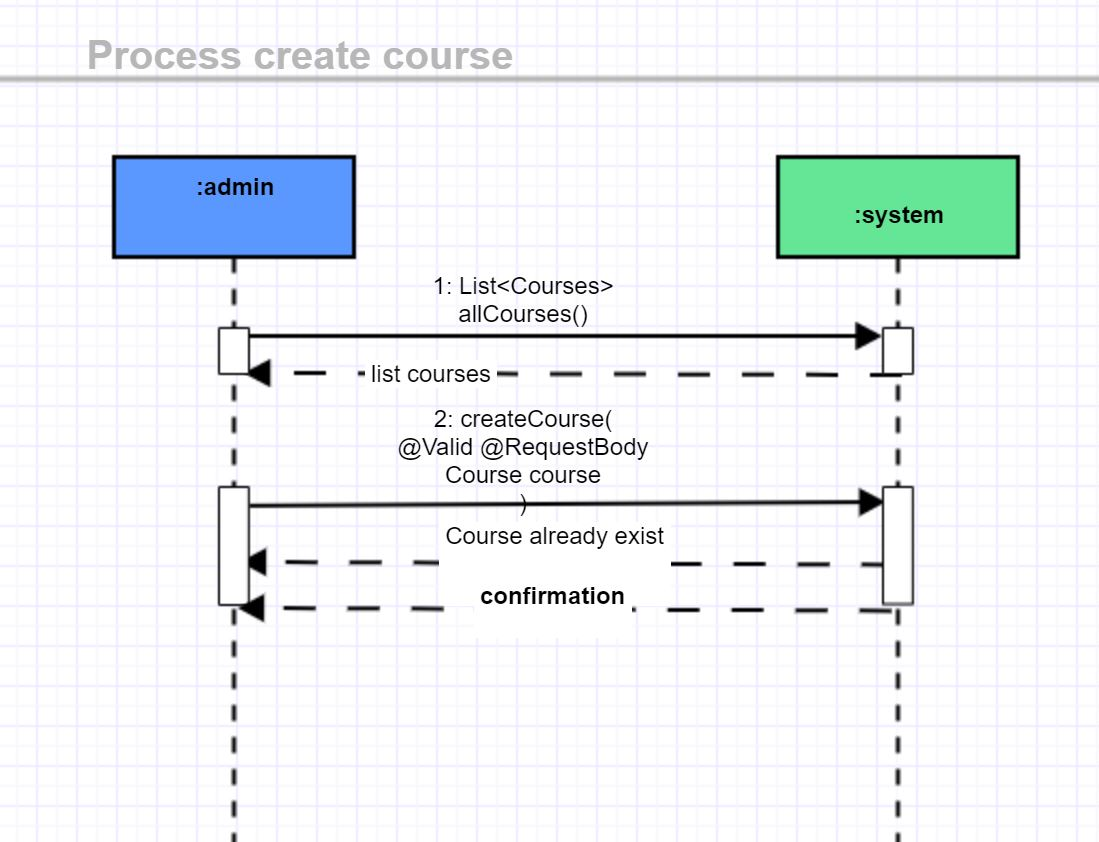
\includegraphics[width = 100mm]{sd/sd-createCourse}
\caption{sd for create a course }
\label{sd for create a course}
\end{figure}

Use case "Manage offering Courses"\\
\textbf{Update a course}
\begin{figure}[H]
\centering
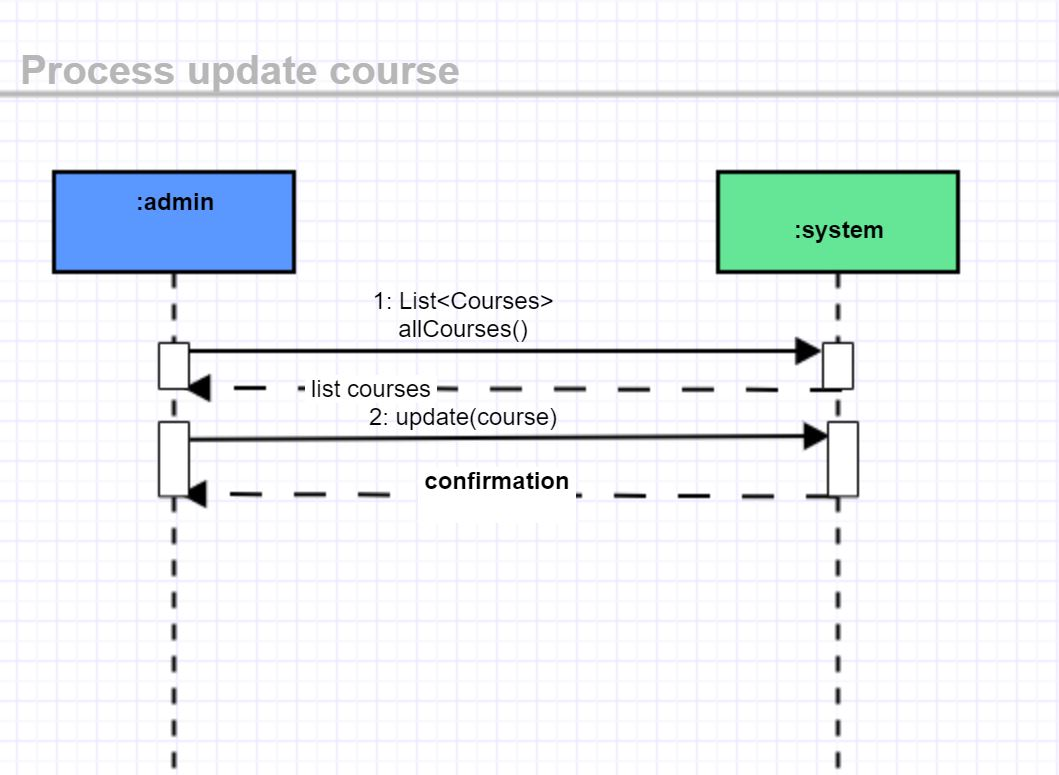
\includegraphics[width = 100mm]{sd/sd-updateCourse}
\caption{sd for create a course }
\label{sd for update a course}
\end{figure}

\newpage
Use case "Manage offering Courses"\\
\textbf{Delete a course}
\begin{figure}[H]
\centering
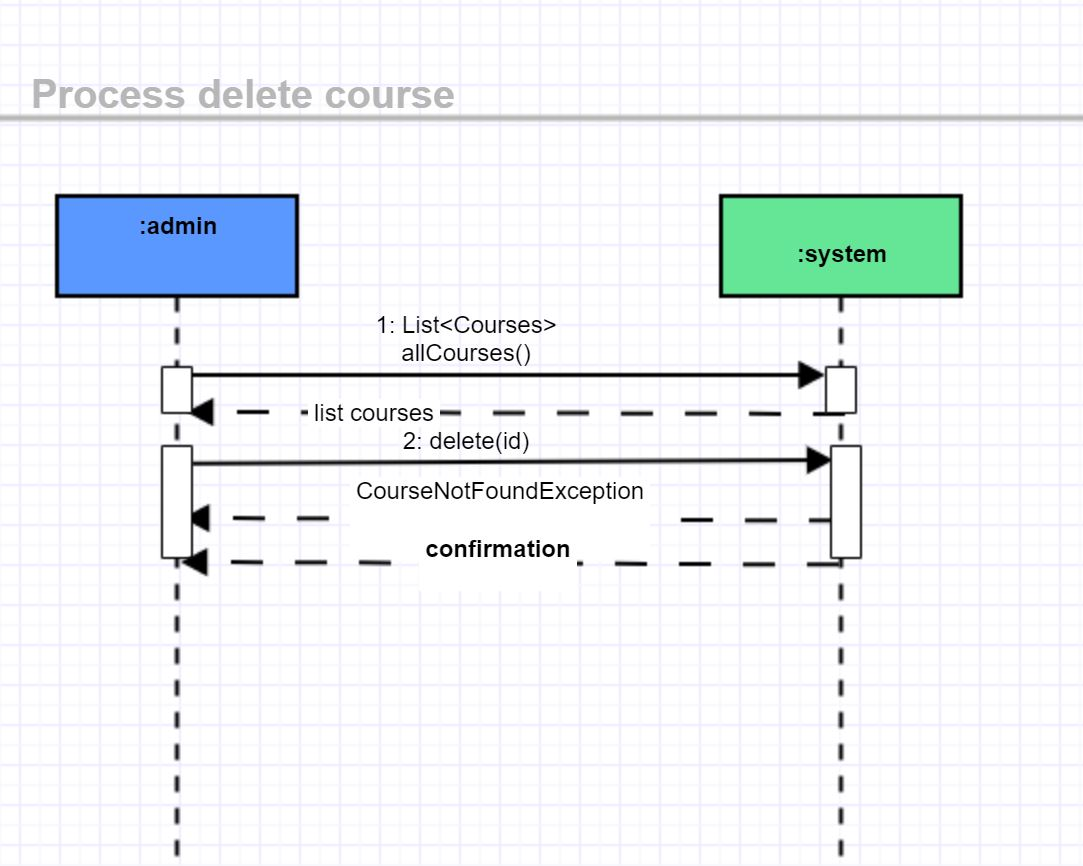
\includegraphics[width = 100mm]{sd/sd-deleteCourse}
\caption{sd for create a course }
\label{sd for delete a course}
\end{figure}

% use case user add a course
Use case "Course registration"\\

\begin{figure}[H]
\centering
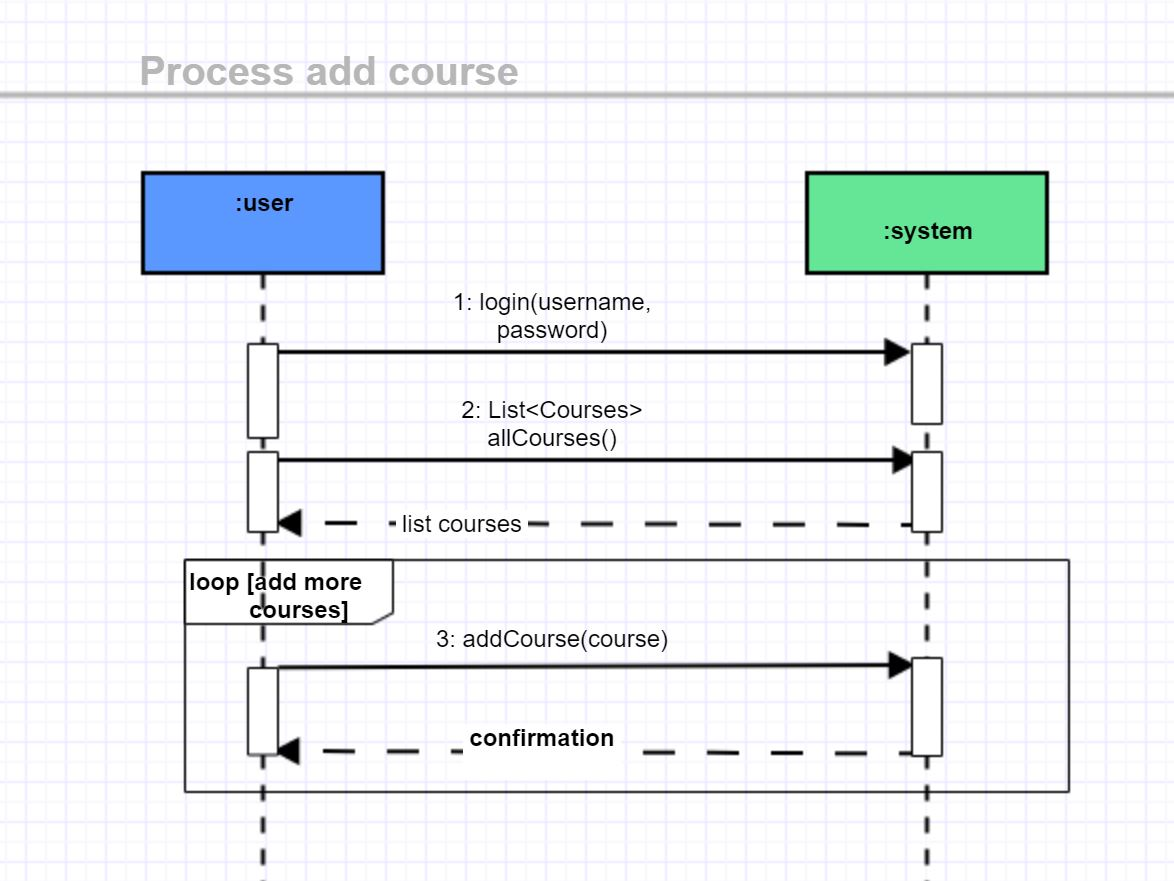
\includegraphics[width = 100mm]{sd/sd-addCourse}
\caption{sd for create a course }
\label{sd for course registration}
\end{figure}

\newpage
%use case exam registration
Use case "Exam registration"\\
\begin{figure}[H]
\centering
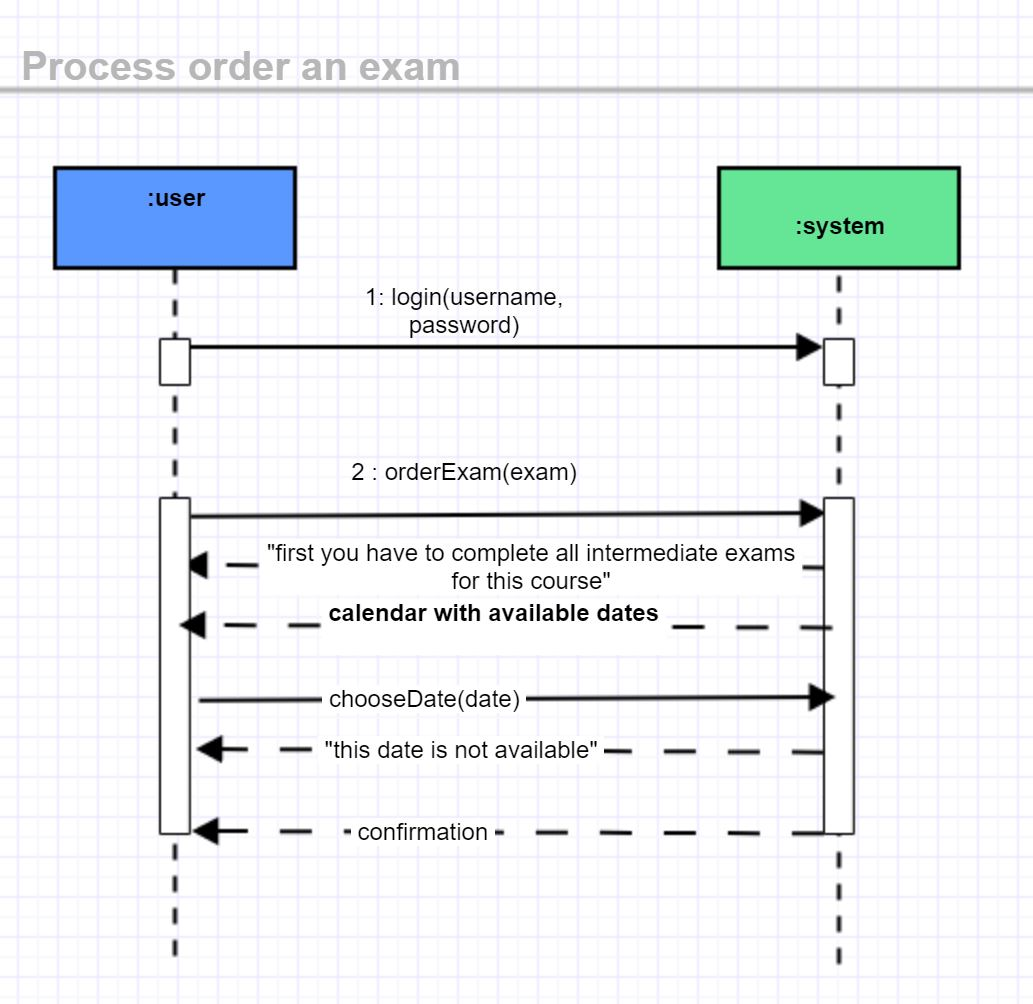
\includegraphics[width = 100mm]{sd/sd-orderExam}
\caption{sd for create a course }
\label{sd for exam registration}
\end{figure}

\subsubsection{Interface viewpoint}
\textbf{\textit{DESIGN CONCERNS}}
\\
The interface viewpoint provides information about how we want to design our user interface. \\

%todo: make and put here the welcome page 
After downloading the application, and running the first time, the user will be directed to Welcome page.\\

\textbf{\textit{Design elements.}}
\textbf{\textit{Catalog page.}}
After click of catalog of courses in the bar menu user will be redirected to Course page.

\begin{figure}[H]
\centering
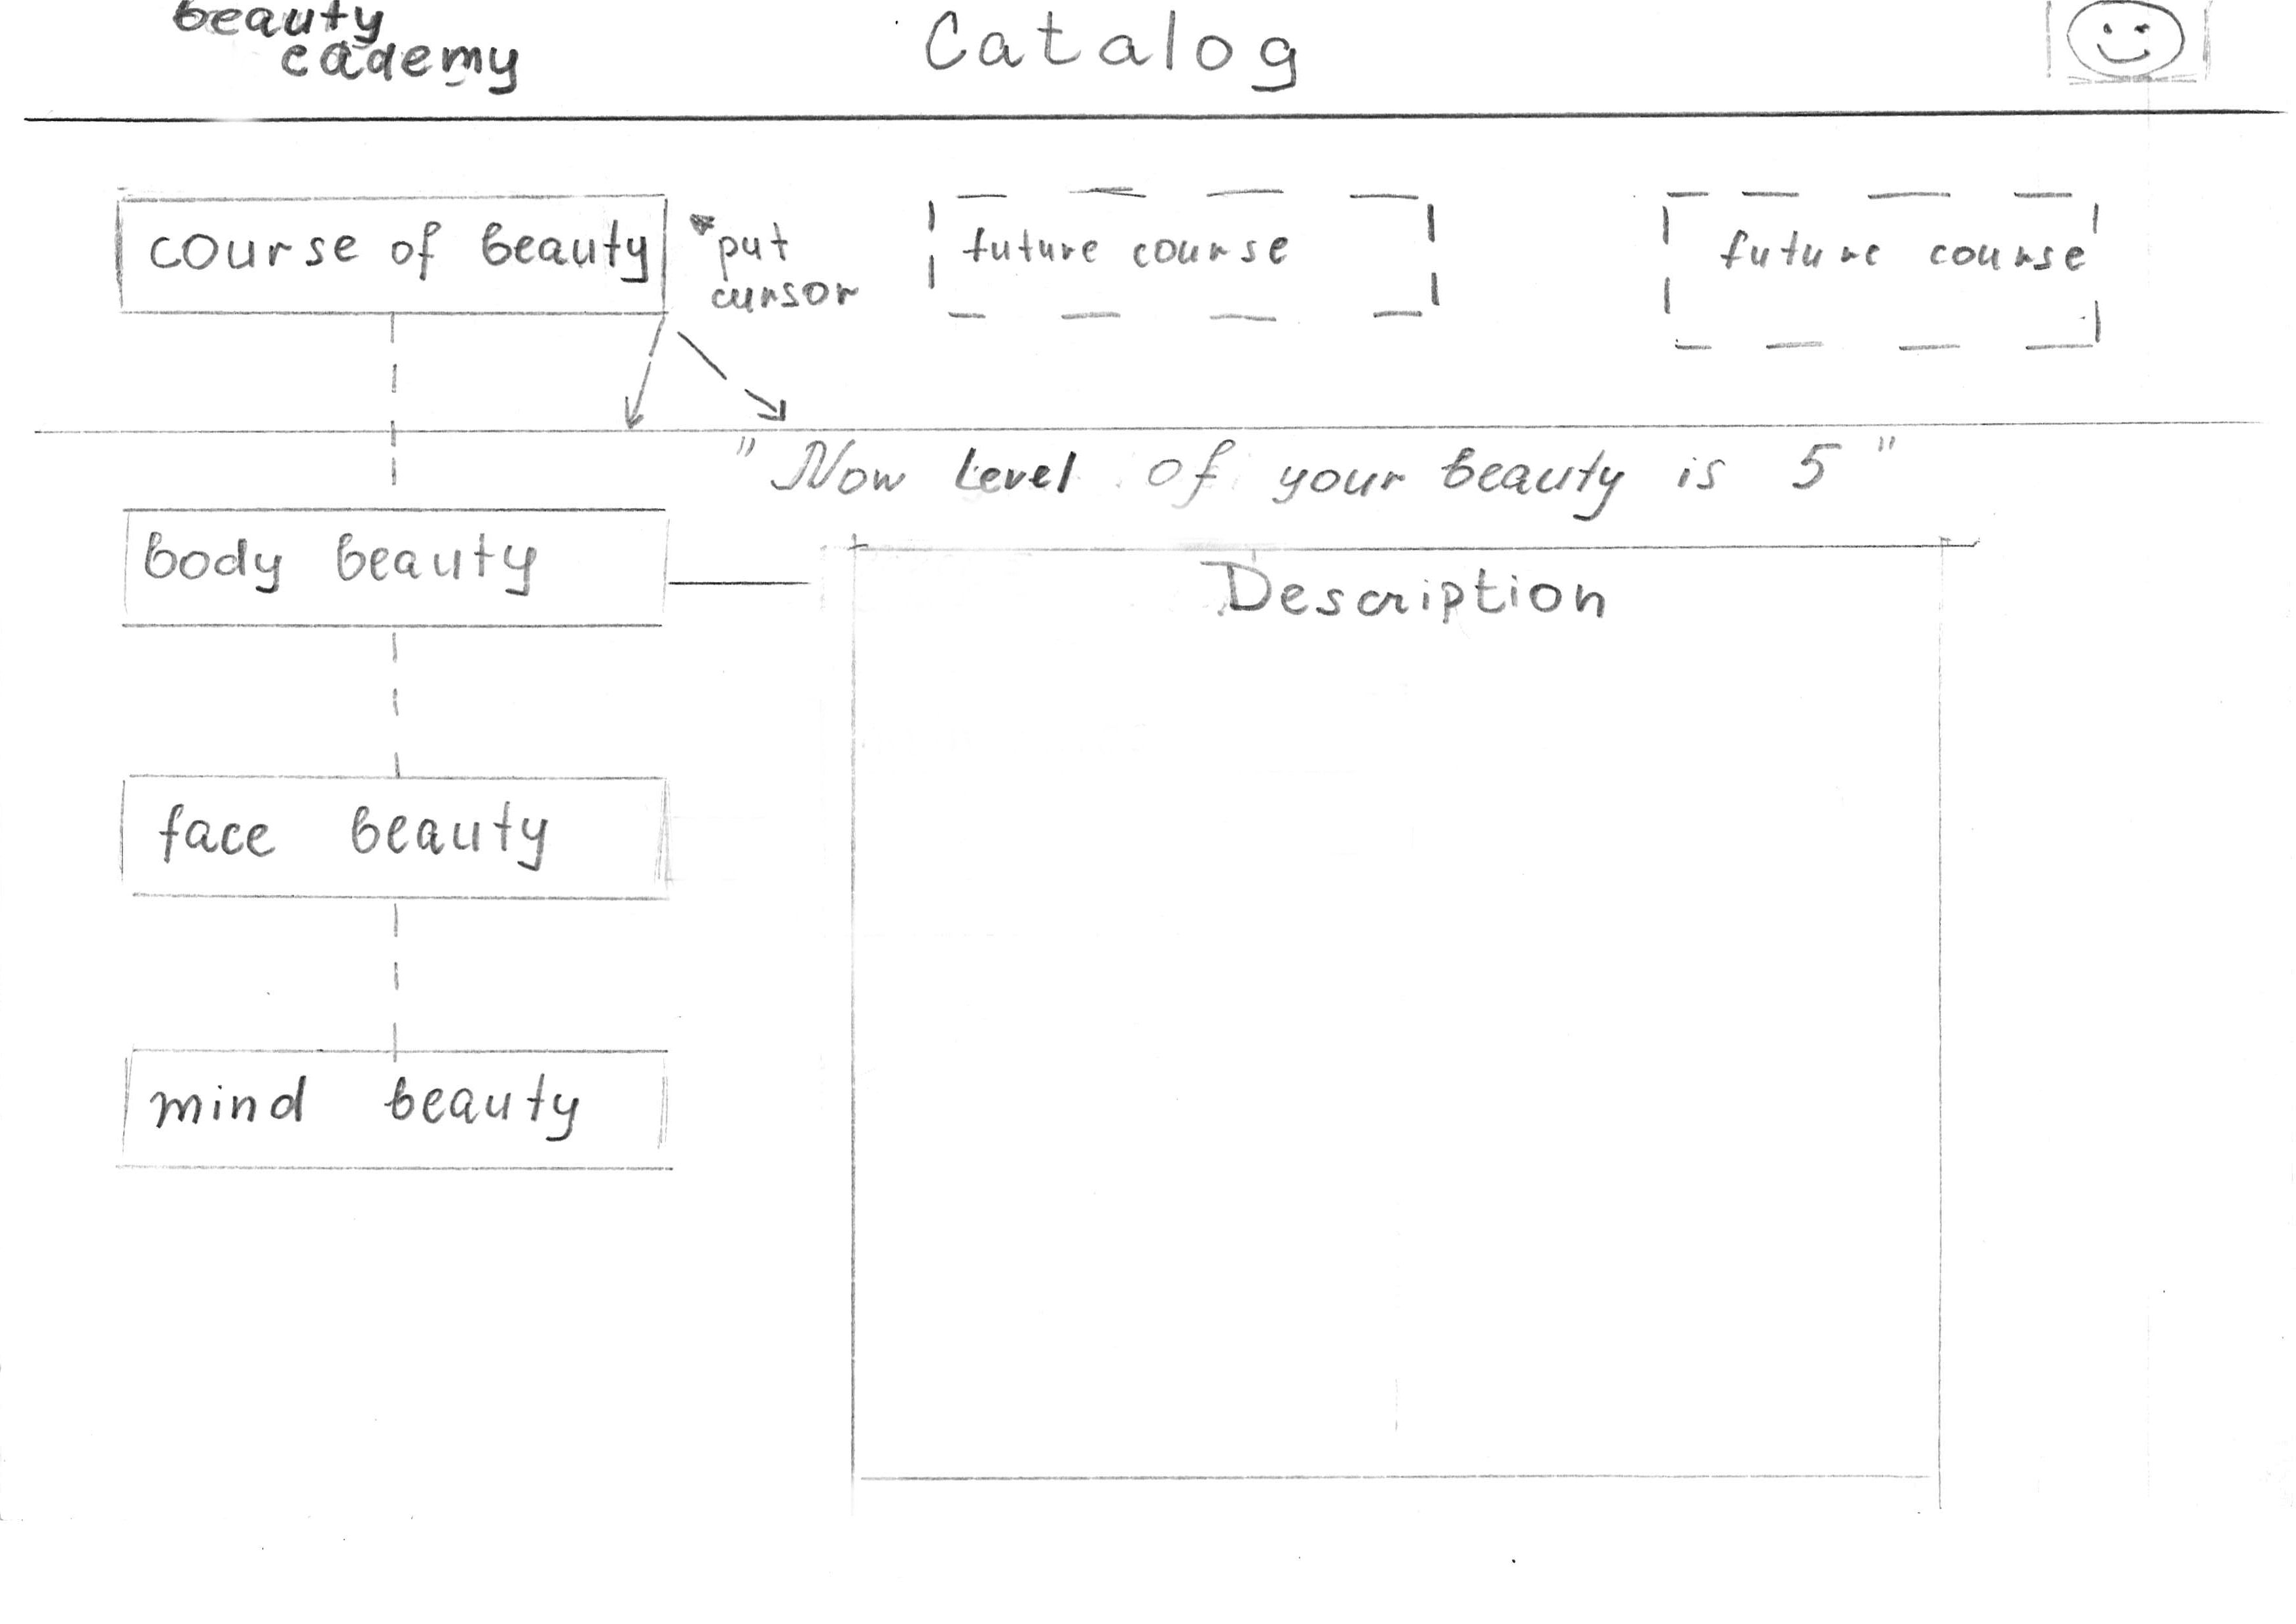
\includegraphics[width = 140mm]{proto-foto/ui-courses.JPG}
\caption{ui design for courses}
\label{welcome page}
\end{figure}

\newpage
\textbf{\textit{Design elements.}}
\textbf{\textit{Login page. }}
After clicking subscription button user will be redirected to the login page.
\begin{figure}[H]
\centering
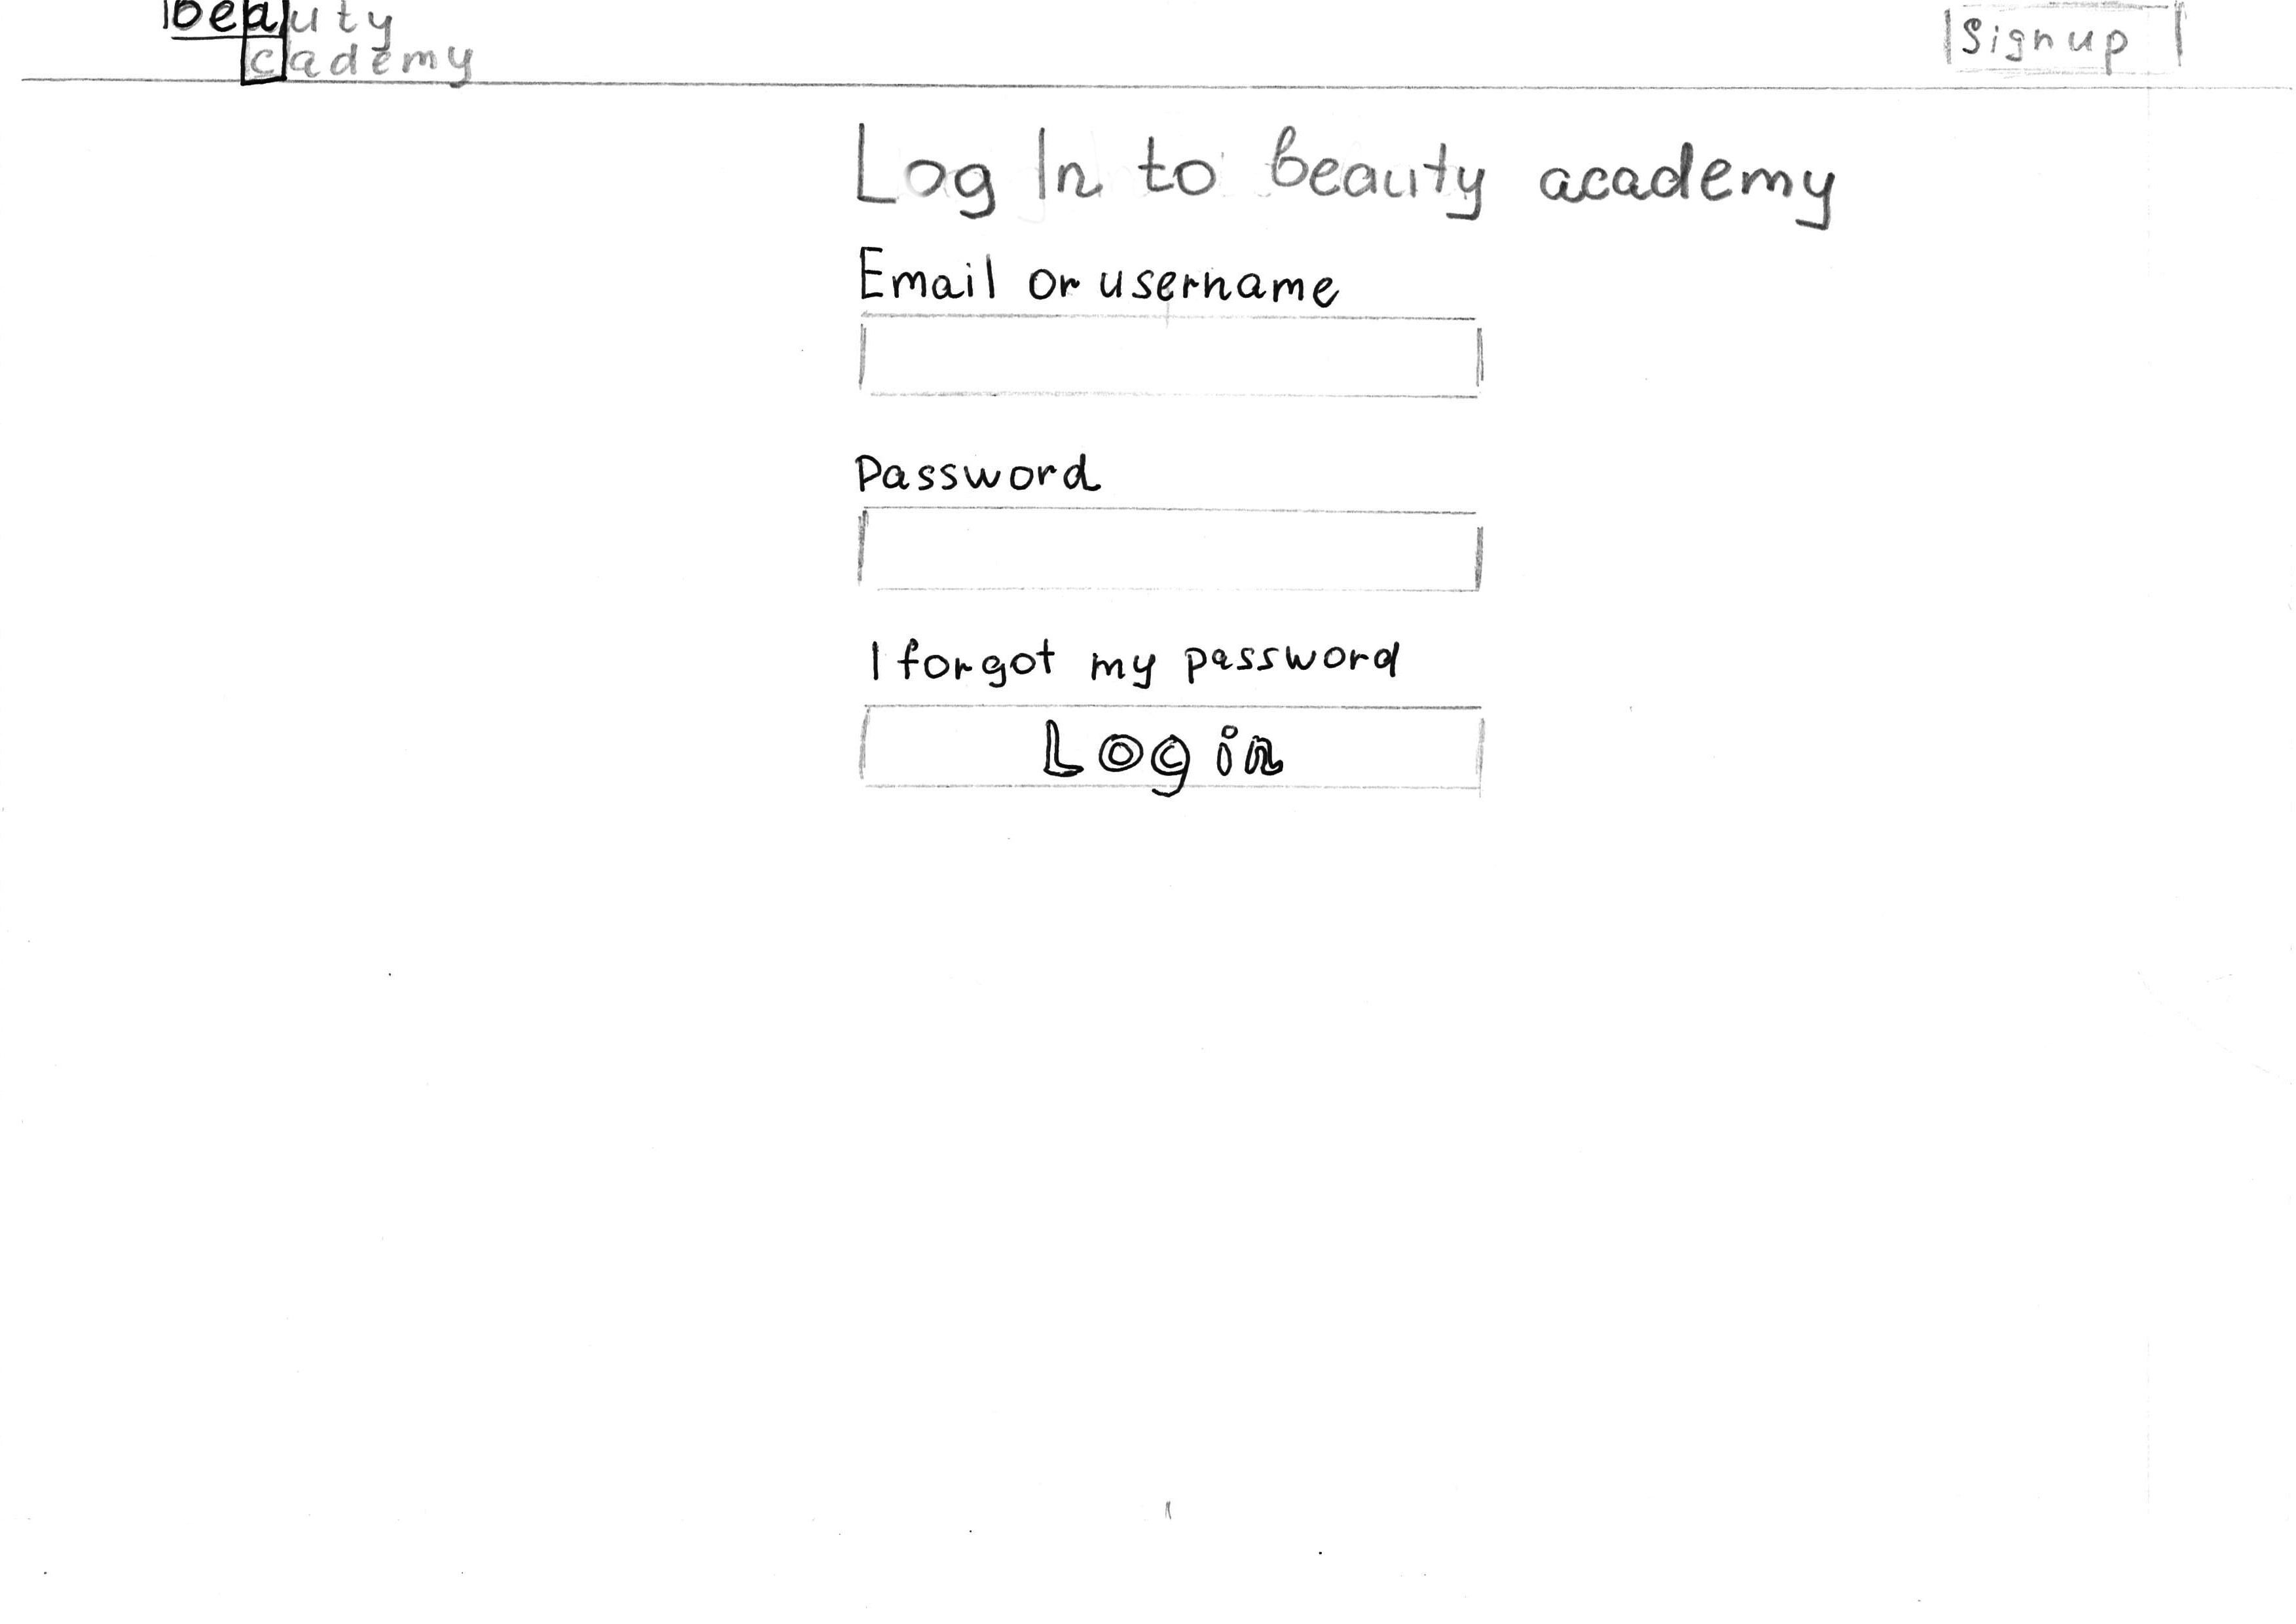
\includegraphics[width = 140mm]{proto-foto/ui-login.JPG}
\caption{ui design for login}
\label{login page}
\end{figure}

\newpage
\textbf{\textit{Design elements.}}
\textbf{\textit{Registration page.}}
After clicking of Sign up button the user will be redirected to the registration page.\\
\begin{figure}[H]
\centering
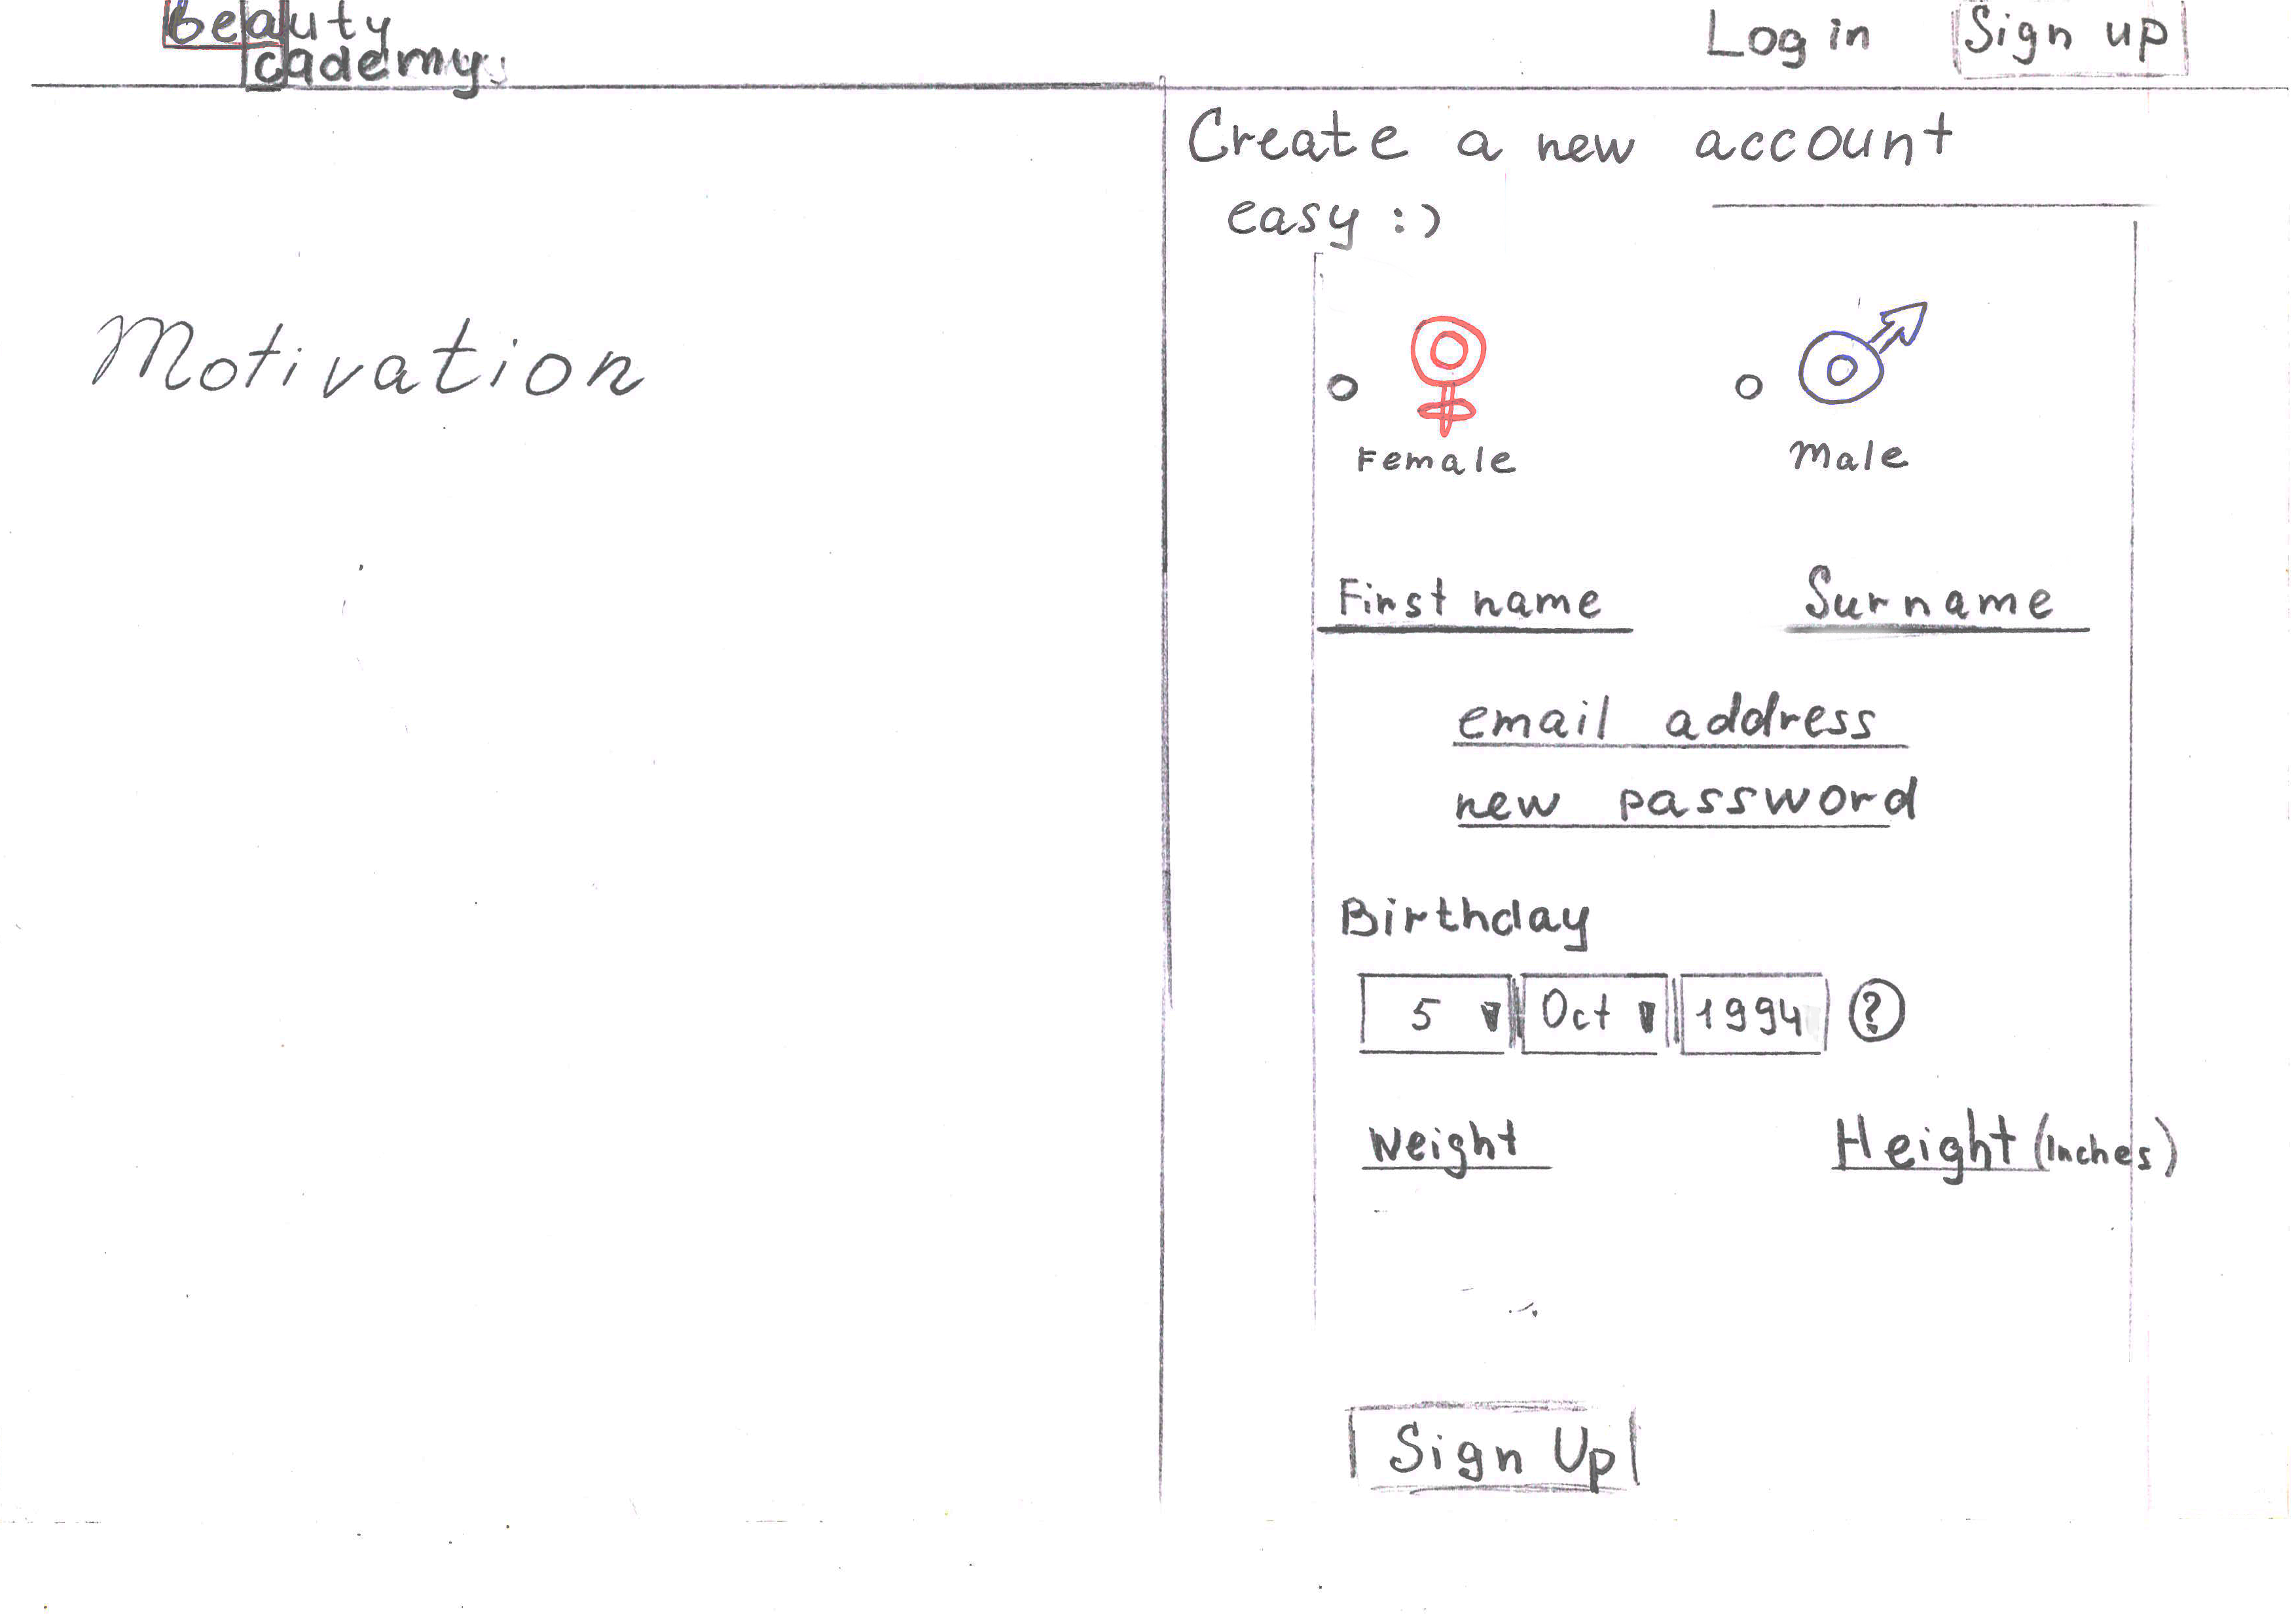
\includegraphics[width = 140mm]{proto-foto/ui-reg.JPG}
\caption{ui design for registration page}
\label{registration page}
\end{figure}

\newpage
\textbf{\textit{Design elements.}}
\textbf{\textit{User page.}}
This is the user page. This page will be have the information about user, courses that he has, etc.//
\begin{figure}[H]
\centering
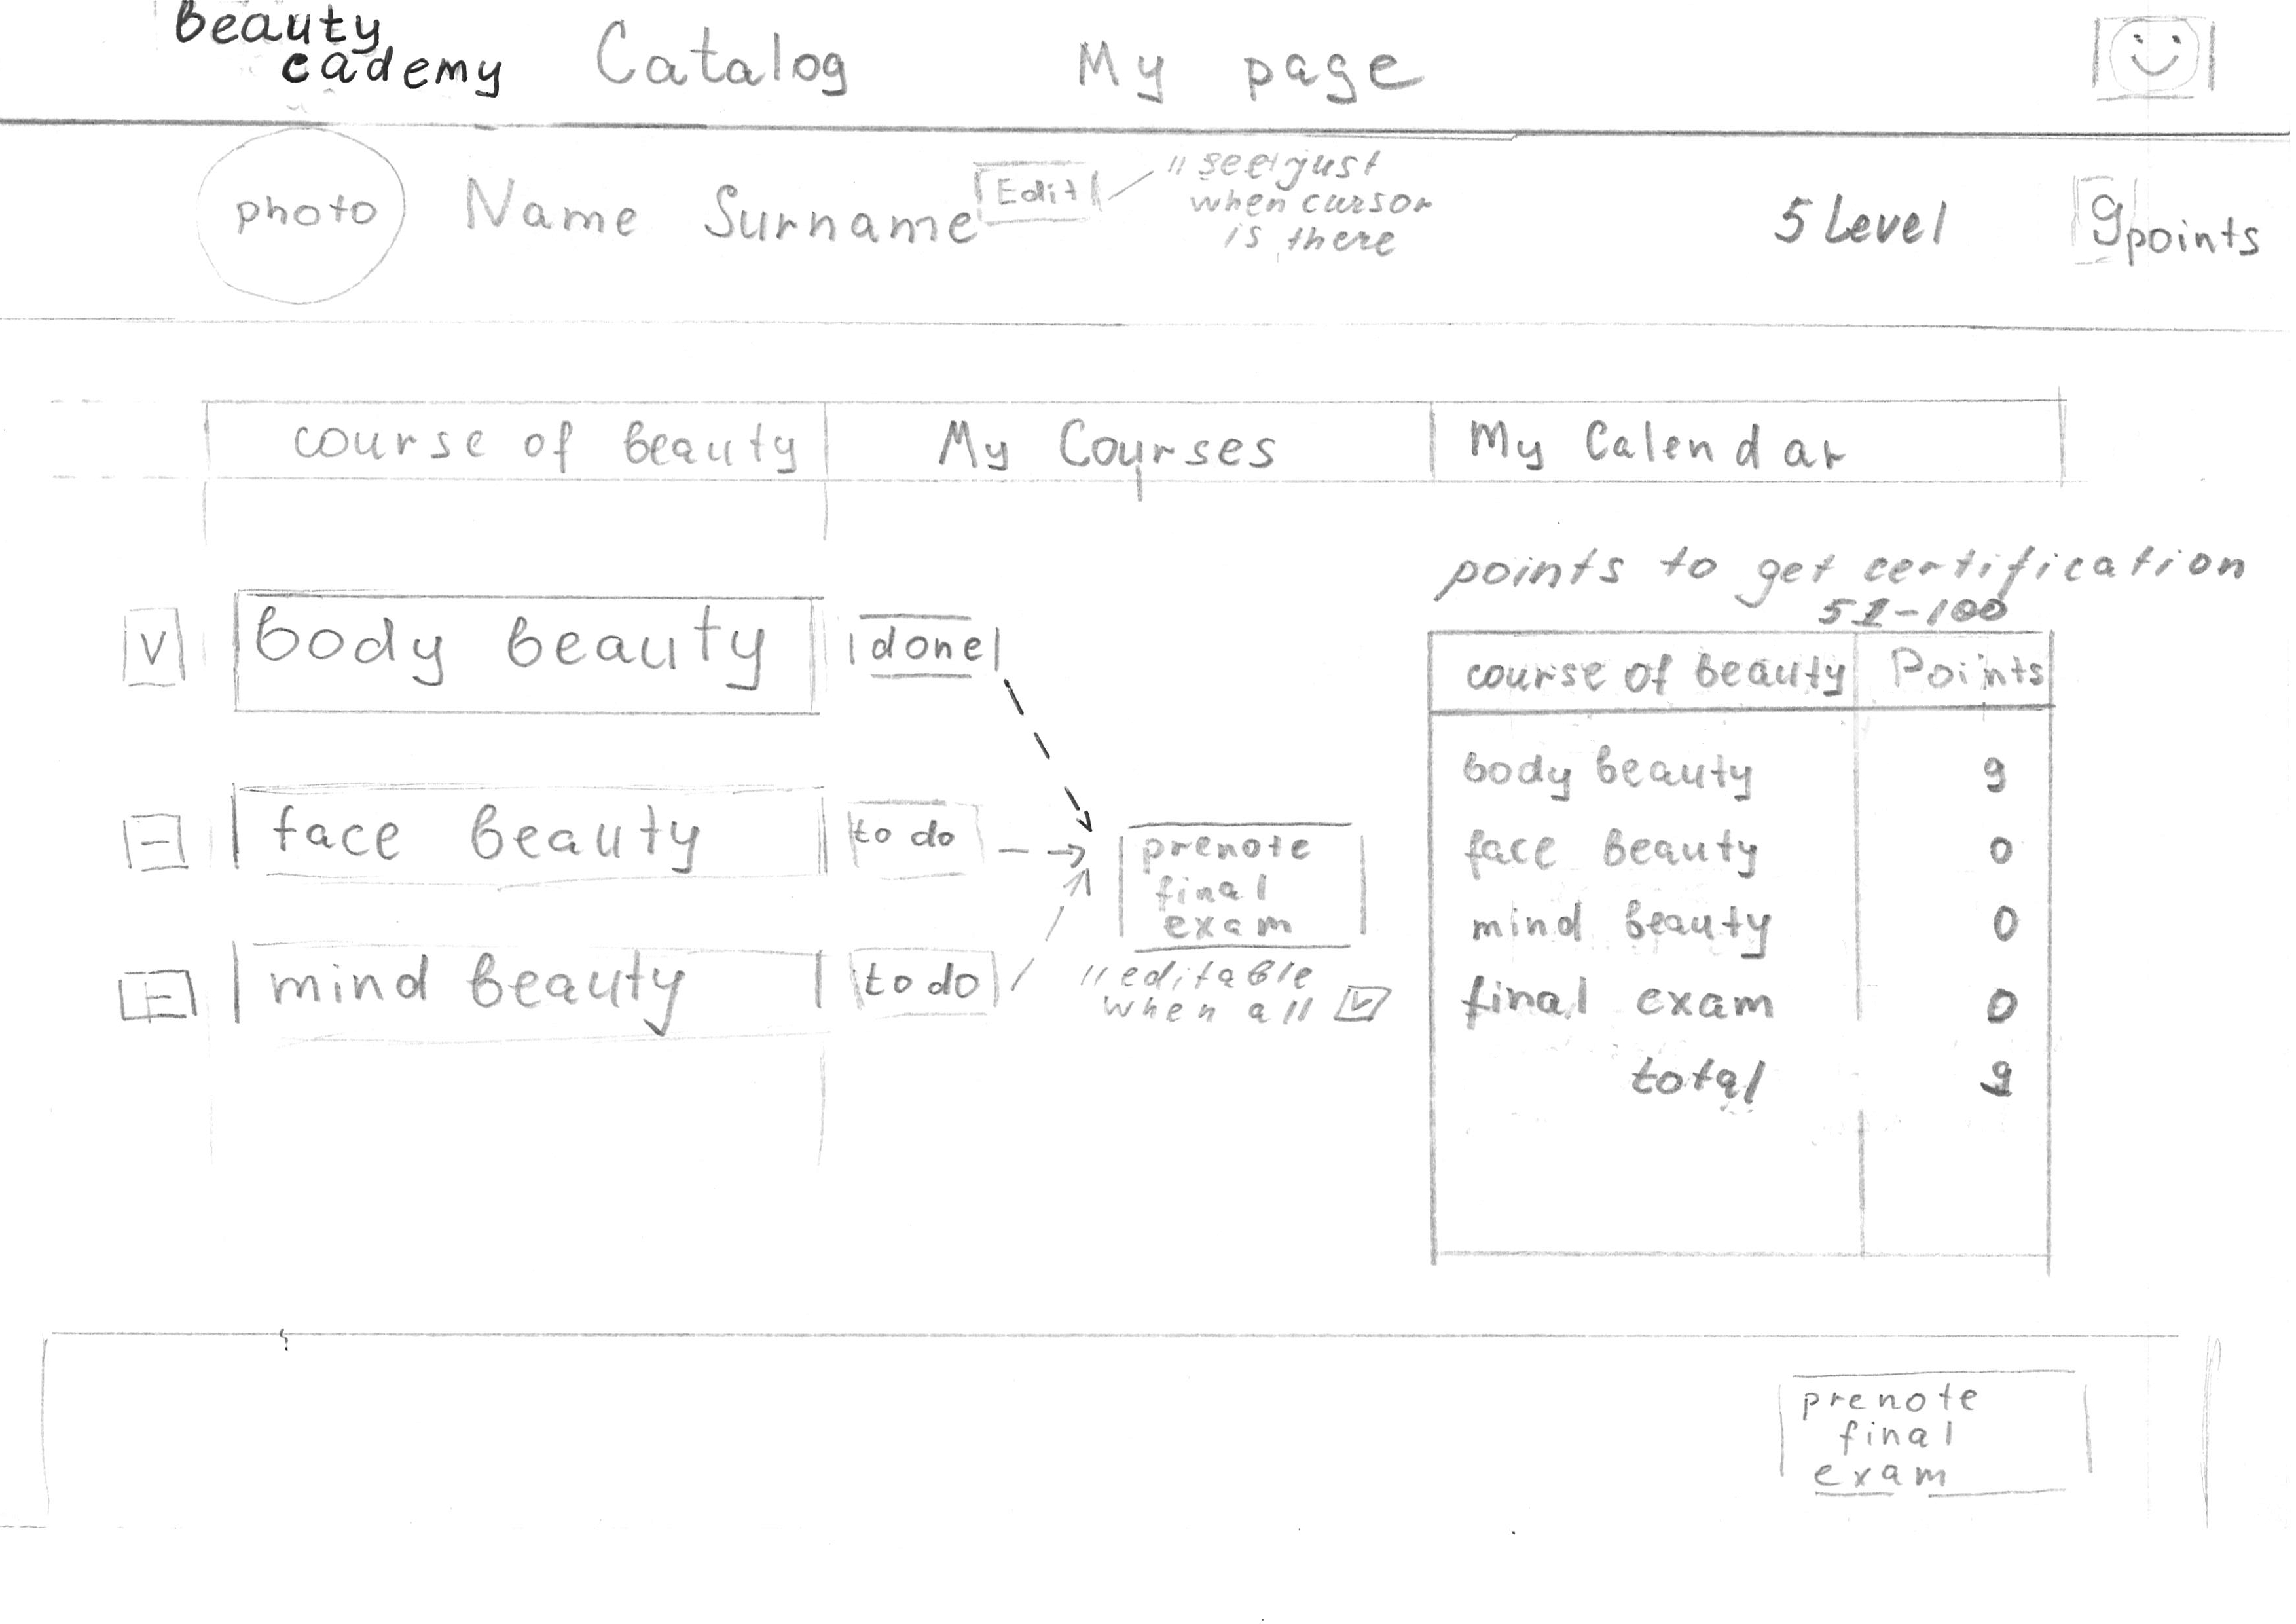
\includegraphics[width = 140mm]{proto-foto/ui-user-page.JPG}
\caption{ui design for profile page}
\label{user page}
\end{figure}

\newpage
\textbf{\textit{Design elements.}}
\textbf{\textit{Topics page.}}
This page is sub page of the courses.
\begin{figure}[H]
\centering
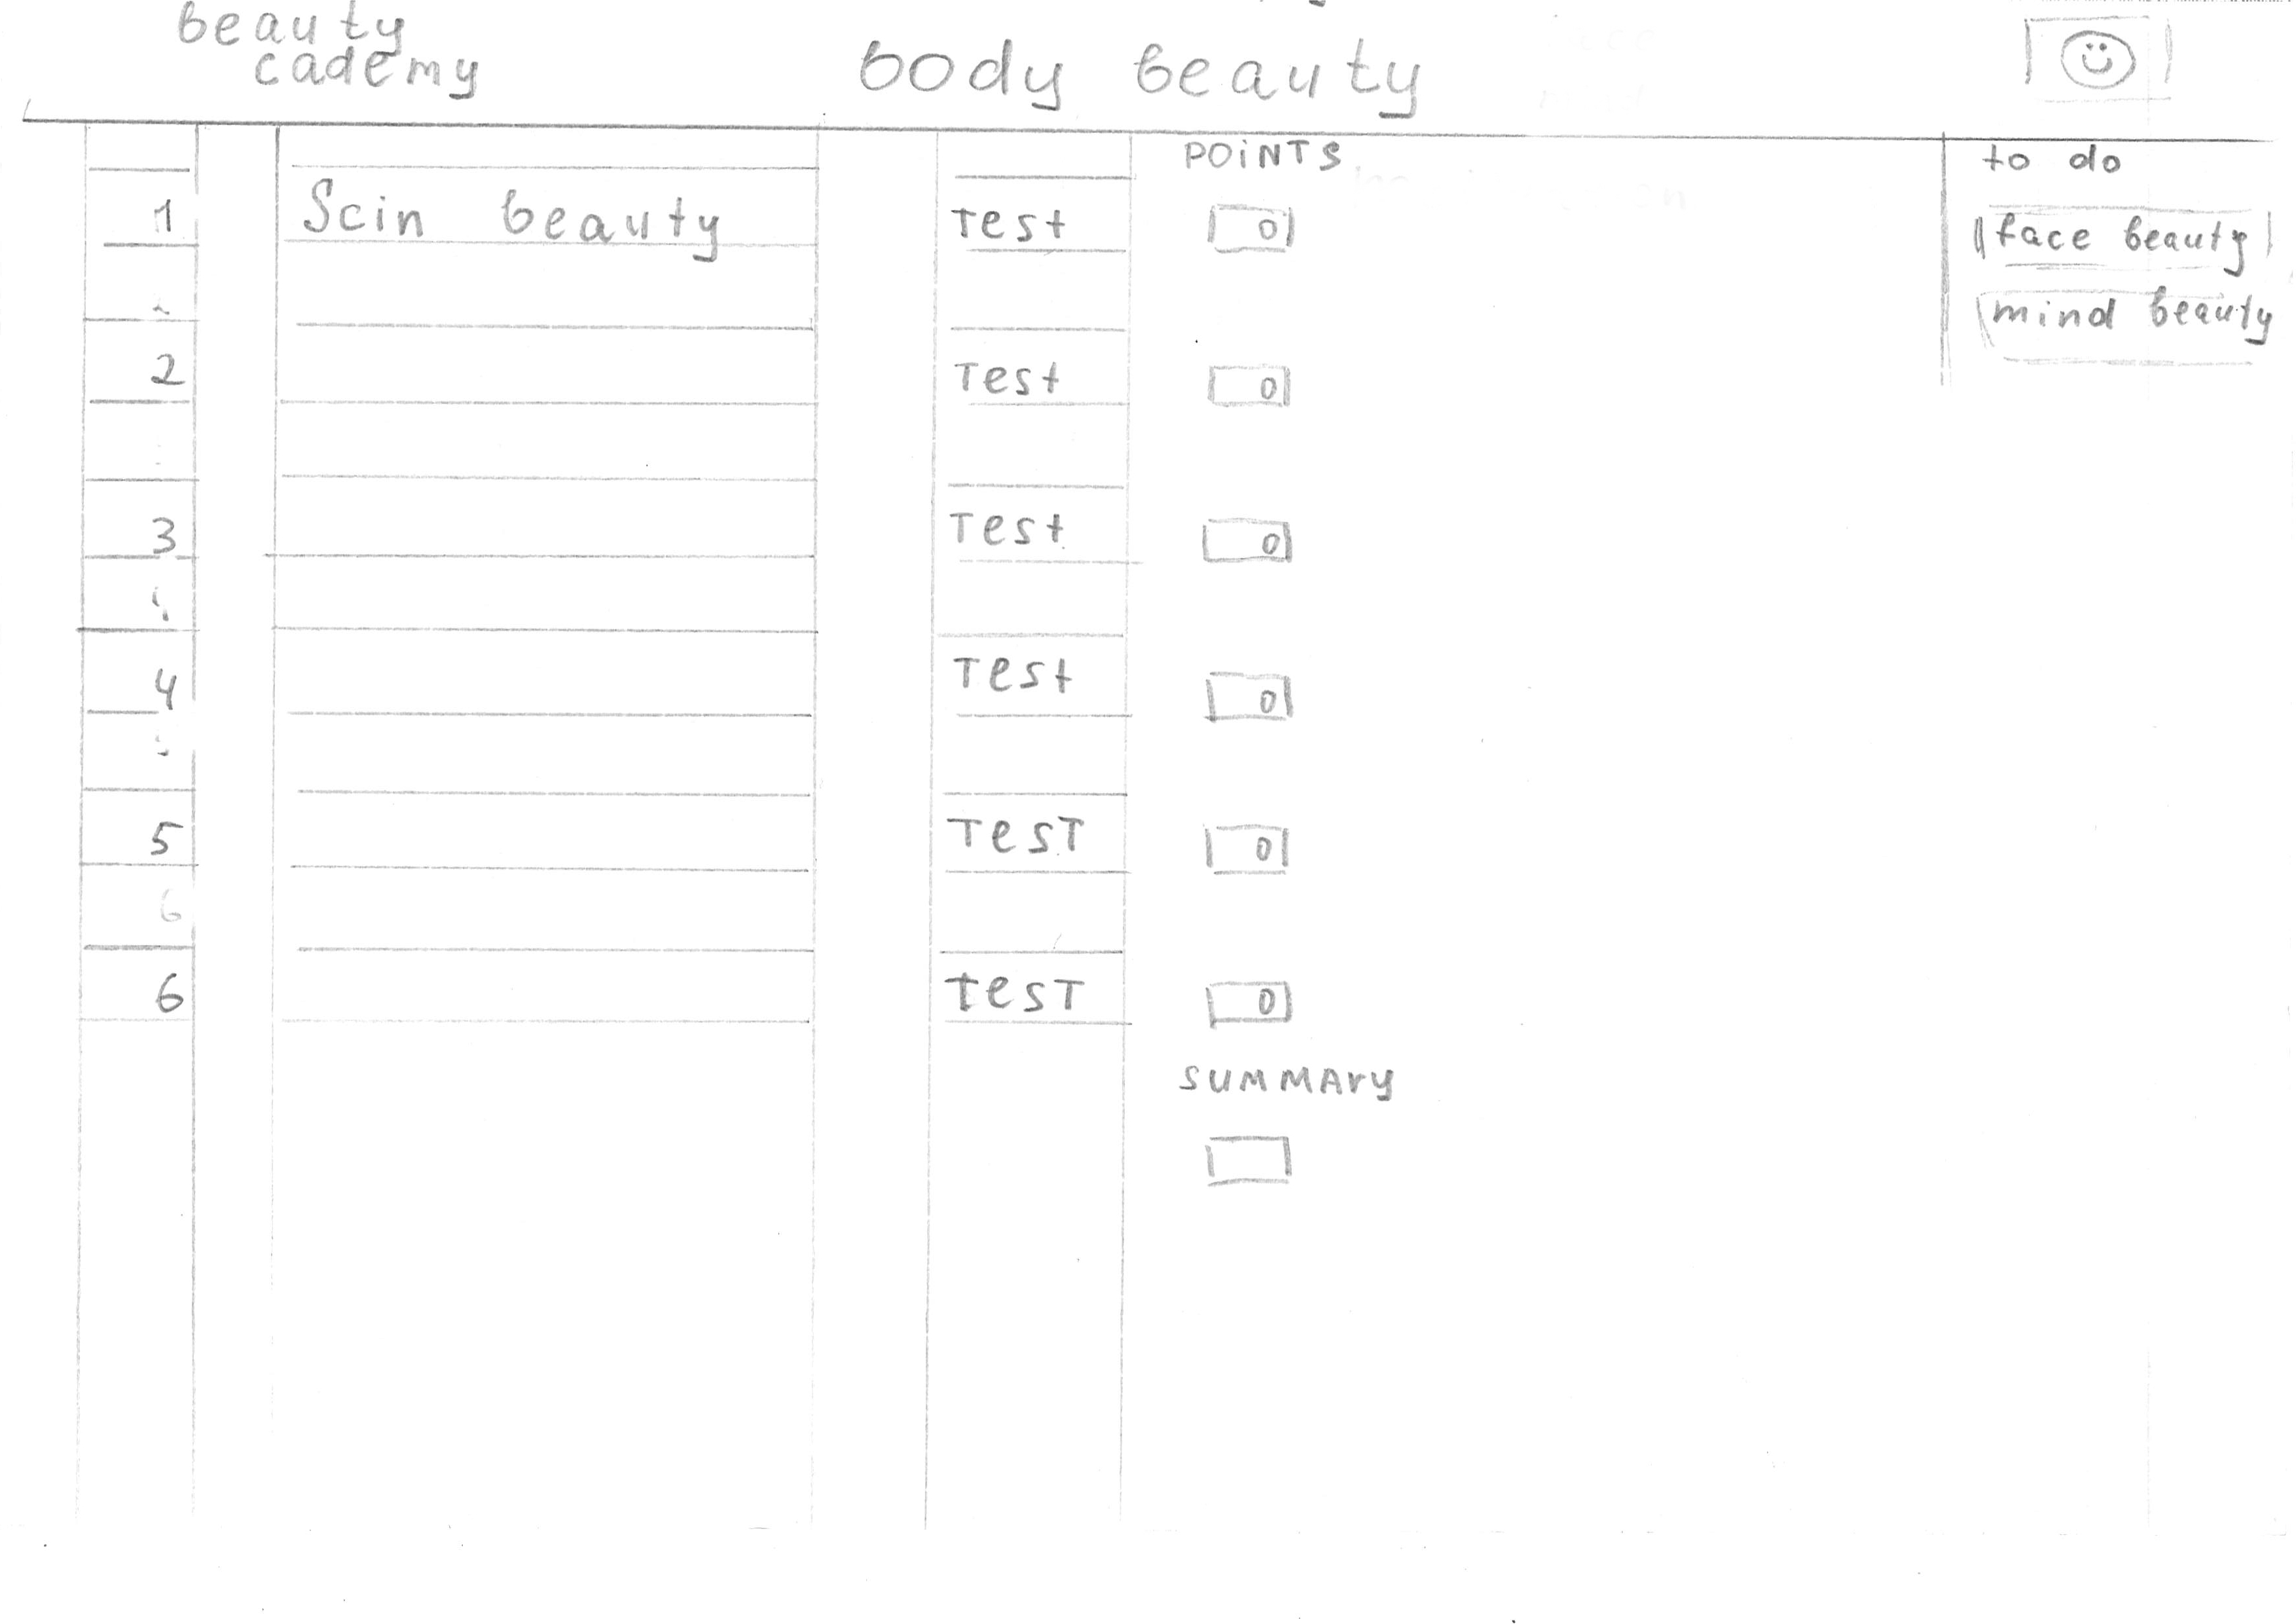
\includegraphics[width = 140mm]{proto-foto/ui-test-topic.JPG}
\caption{ui design for topic with tests}
\label{topics page}
\end{figure}


\subsection{Implementation}
\textbf{\textit{First steps}}\\
First of all want to describe database that I will use.\\
\textbf{PostgreSQL} is a free and open-soursce relational database management system emphasing extensibility and technical standarts compliance. It is designed to handle a range of workloads, from single machines to data warehouses or Web services with many concurrent users. It is the default database for macOS Server, and is also available for Linux, FreeBSD, OpenBSD, and Windows \cite{wiki-posgres}.\\

 I  will use \textbf{Maven} as tool to build our project. The layers have to be independently deployable components, with  their own vesions, depending between them and making up a whole application. This description fits with \textbf{Maven modules}.\\
 First, I need a maven project with packaging type “pom”. Then, I'll add each layer as a module to this maven project. Once I’ve  done this, I can add the dependencies between layers.\\
 Then I need some Spring dependencies to make this project works.\\
 These are the Spring dependencies required in each layer:\\
\textbf{-boot}: spring-core, spring-beans, spring-context, spring-boot, spring-boot-autoconfigure     	and spring-boot-starter-undertow.
\textbf{presentation}: spring-webmvc and spring-beans.\\
\textbf{application}: spring-context.\\

Here I want to describe the concern of each layer.
\textbf{\textit{Backend }}


\begin{itemize}
\item Integration/ Data layer (entity models and repository)
\textbf{Domain}
In this layer I save:
These are the \textbf{entities} which represents the domain. This is the heart of our application, so the domain layer has to be isolated and it can't depend on another layer of the application.\\
\textbf{Repository}
@Repository is a Spring annotation that indicates that the decorated class is a repository. A repository is a mechanism for encapsulating storage, retrieval, and search behaviour which emulates a collection of objects. It is a specialization of the @Component annotation allowing for implementation classes to be autodetected through classpath scanning.	
	
\item	Application/ Service layer \\
Service layer or business layer, based on the User command and the data captured from the user. It takes a domain-specific decision, like what to do with the data, which table to look, how to manipulate the data which comes from the database, so it can be presented in UI.\\
The services are the most important pieces of this layer, they orchestrate the domain objects to fulfil a use case. Another important thing is done inside these services are the translation from raw data to the domain model.\\
\item  Web layer or presentation layer\\
This layer interacts with the end-user, shows data to them, take user input, take command from them, etc.

\item Boot \\
Boot layer is required one in our application with Spring. This layer depends on every other layer previously mentioned and stores the MainApplication class which starts the Spring Boot application. Because it depends on the other layers, Spring dependency injection mechanism can inject the annotated components of the other layers. It’s important to know that only the components in the same package (or subpackages) of the MainApplication class are scanned. The generated jar of this Maven module will be the executable one, the other modules are libraries in which this module depends on.\\


\end{itemize}

\textbf{What is restful?}
Building REST services with Spring
REST has quickly become the de-facto standard for building web services on the web because they’re easy to build and easy to consume.\\
\textbf{Why REST?} REST embraces the precepts of the web, including its architecture, benefits, and everything else.
What \textbf{benefits}? The web and its core protocol, HTTP, provide a stack of features:\\
Suitable actions (GET, POST, PUT, DELETE, …​)\\
Caching\\
Redirection and forwarding\\
Security (encryption and authentication)\\

So building on top of HTTP, REST APIs provide the means to build flexible APIs that can:\\
Support backward compatibility\\
Evolvable APIs\\

Scalable services\\

Secure services\\

A spectrum of stateless to stateful services\\


\textbf{\textit{Frontend – Angular }}
The basic building blocks of an Angular application are NgModules, which provide a compilation context for components. NgModules collect related code into functional sets; an Angular app is defined by a set of NgModules. Our app has  root module that enables bootstrapping.\\

 - Components define views, which are sets of screen elements that Angular can choose among and modify according to your program logic and data.\\

 - Components use services, which provide specific functionality not directly related to views. Service providers can be injected into components as dependencies, making your code modular, reusable, and efficient.\\

Both components and services are simply classes, with decorators that mark their type and provide metadata that tells Angular how to use them.\\

 - The metadata for a component class associates it with a template that defines a view. A template combines ordinary HTML with Angular directives and binding markup that allow Angular to modify the HTML before rendering it for display.\\

 - The metadata for a service class provides the information Angular needs to make it available to components through dependency injection (DI).\\

An app's components define many views, arranged hierarchically. Angular provides the Router service to help us define navigation paths among views. The router provides sophisticated in-browser navigational capabilities.\\

\textbf{Modules} \\
Angular NgModules differ from and complement JavaScript (ES2015) modules. An NgModule declares a compilation context for a set of components that is dedicated to an application domain, a workflow, or a closely related set of capabilities. An NgModule associate its components with related code, such as services, to form functional units.\\

Every Angular app has a root module, conventionally named AppModule, which provides the bootstrap mechanism that launches the application. An app typically contains many functional modules.\\


\textbf{Components}\\
This application has many components and the root component that connects a component hierarchy with the page document object model (DOM). Each component defines a class that contains application data and logic, and is associated with an HTML template that defines a view to be displayed in a target environment.\\

The @Component() decorator identifies the class immediately below it as a component, and provides the template and related component-specific metadata.\\

\textbf{Templates}\\
A template combines HTML with Angular markup that can modify HTML elements before they are displayed. Template directives provide program logic, and binding markup connects your application data and the DOM. \\

\textbf{Services and dependency injection}\\
For data or logic that isn't associated with a specific view, and that you want to share across components, we have created. A service class is preceded by the @Injectable() decorator. The decorator provides the metadata that allows other providers to be injected as dependencies into our class.\\
\\
Dependency injection (DI) lets us keep our component classes lean and efficient. They don't fetch data from the server, validate user input, or log directly to the console; they delegate such tasks to services.\\

\textbf{Routing}\\
The Angular Router NgModule provides a service that lets us define a navigation path among the different application states and view hierarchies in your app. It is modelled on the familiar browser navigation conventions.\\
The router maps URL-like paths to views instead of pages. When a user performs an action, such as clicking a link, that would load a new page in the browser, the router intercepts the browser's behaviour, and shows or hides view hierarchies.\\




\begin{itemize}
	\item	Angular MVC Framework by Google
	\item	Component-based
	\item	Main programming Language is Typescript
	\item	Own structure
	\item	CSS (Design the GUI)
	\item   Angular Material Design

\end{itemize}
\begin{figure}[H]
\centering
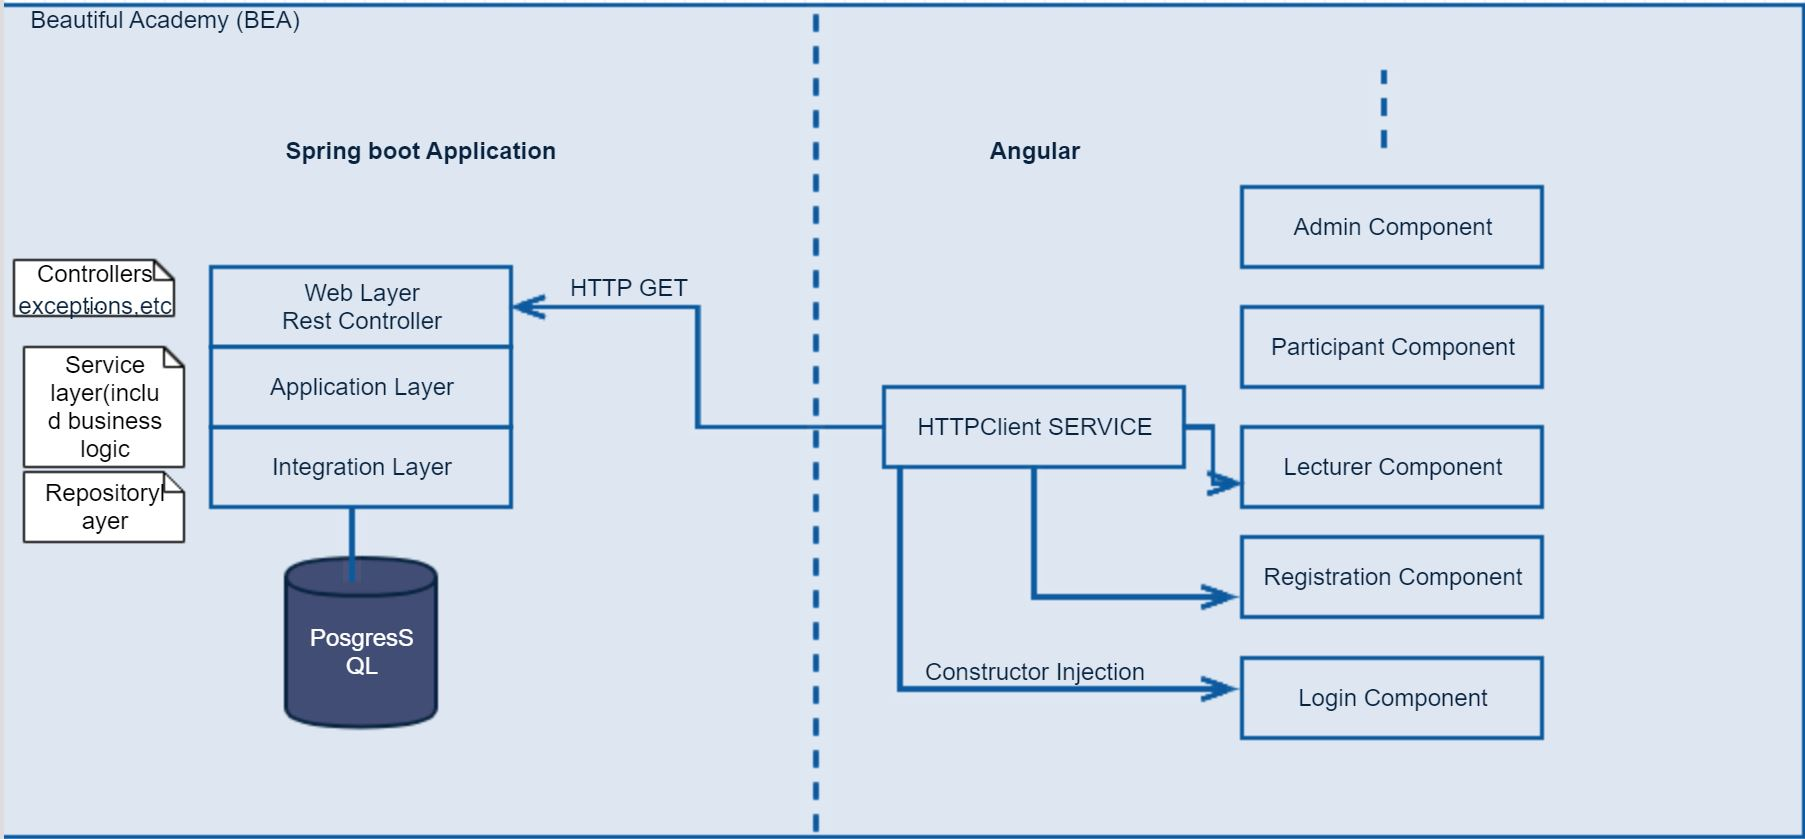
\includegraphics[width = 130mm]{layer.JPG}
\caption{Layer model of application implementation}
\label{layers}
\end{figure}

\subsubsection{Why Spring Boot And Angular ?}
\textbf{BUILD Backend WITH SPRING BOOT}\\
Before starting with spring boot, it was clear for me about spring boot that spring boot does not provide any extra features on functionality on top of spring framework. Rather, it provides unlimited defaults configurations and useful conventions to create a stand-lone, production-grade web application in no time.\\
Spring Boot is the starting point for building all Spring-based applications. Spring Boot is designed to get you up and running as quickly as possible, with the minimal upfront configuration of Spring.\\
 -Get started in seconds using Spring Initializer\\
-Build anything: REST API, WebSocket, web, streaming, tasks, and more\\
-Simplified security\\
-Rich support for SQL and NoSQL\\
-Embedded runtime support: Tomcat, Jetty, and Undertow\\
-Developer productivity tools such as Live Reload and Auto Restart\\
-Curated dependencies\\
-Production-ready features such as tracing, metrics, and health status\\
-Works in your favourite IDE: Spring Tool Suite, IntelliJ IDEA, and NetBeans\\

Using these features it has really made building a production-grade Spring applications very easy and faster for developers. Also, no XML configurations required anymore with spring boot\cite{spring-docs}.\\

\textbf{ANGULAR FOR FRONT-END} \\
The technology for front-end is Angular.\\
Angular helps build interactive and dynamic single page applications (SPAs) with its compelling features including templating, two-way binding, modularization, RESTful API handling,\\ dependency injection, and AJAX handling. We can use HTML as template language and even extend HTML’ syntax to easily convey the components of the application.\\
Angular applications are built using TypeScript language, a superscript for JavaScript, which ensures higher security as it supports types (primitives, interfaces, etc.). It helps catch and eliminate errors early when writing the code or performing maintenance tasks.\\
Angular has a lot of pros\\
-simplicity\\
-efficiency\\
- Developers find AngularJS very effective especially in creating dynamic, single page apps, and supporting MVC (Model View Controller) programming structure.\\
-time-saving Projects that previously used to take many months with other frameworks can now be completed faster with AngularJS. All that AngularJS framework requires is splitting the app into several MVC components. From there, the framework takes over because you do not require additional coding.\\
-the app is easy to learn and get started.\\
-data binding in AngularJS is very easy.\\
I like in Angular that it gives our application a clean structure, that is easy to understand and easy to maintain.\\
It brings a lot of utility code that we can reuse, for example, users navigation. Angular applications are more testable \cite{5reason}.\\

\subsubsection{Description of the deployment procedure.}
\textbf{Configuring PosgreSQL}
First, you have to take steps that are described here \url{ https://www.postgresql.org/}\\ You have to create a new database, create a name for it.
 Then you can configure Spring Boot to use PostgreSQL as our data source, you can do that simply by adding PostgreSQL database URL, username, and password in the \textbf{src/main/resources/application.properties} file \\
 
%todo put a photo of application.properties file and maybe file location


 \begin{figure}[H]
\centering
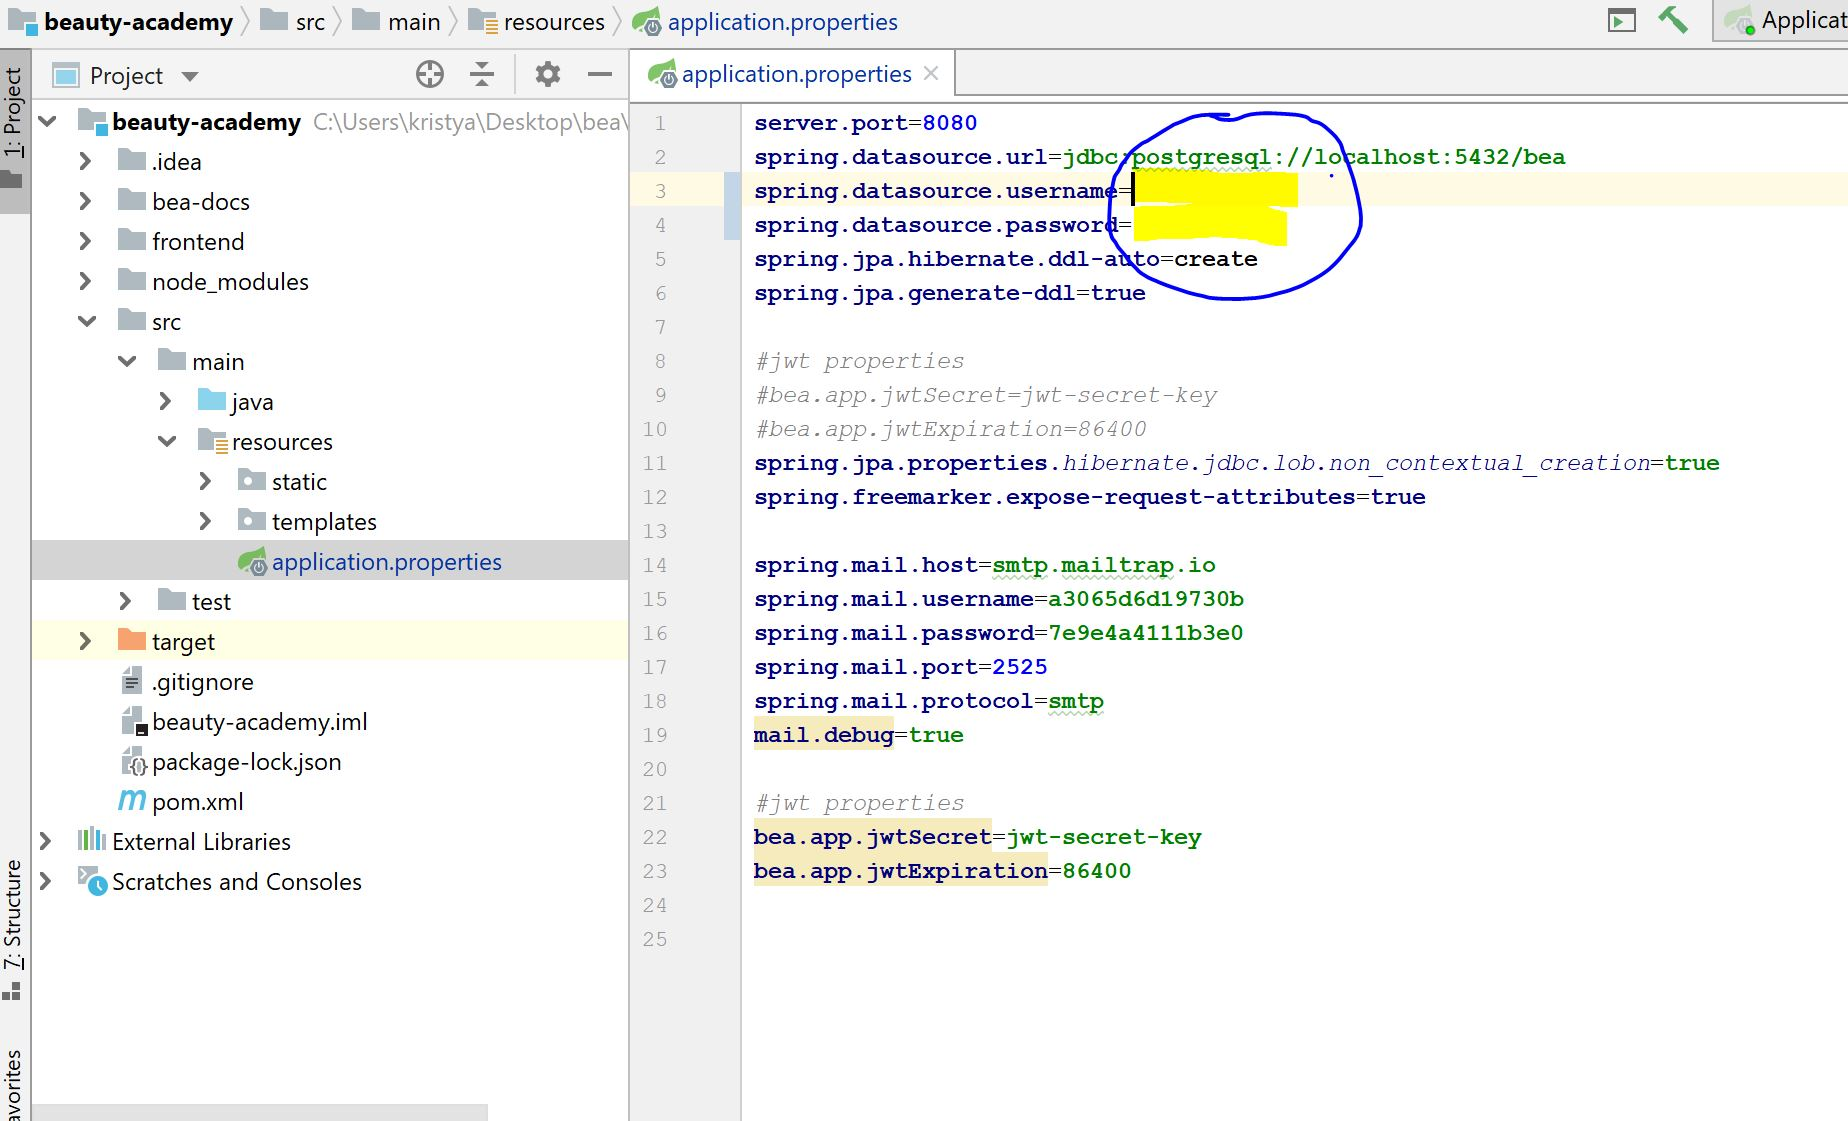
\includegraphics[width=150mm]{application-properties}
\caption{This figure shows how to configure a property file}
\label{blabla}
\end{figure}
 
 Figure 17 shows the application.properties file, that you have to change by putting your username, a password for posgresQL.\\
 
I have used angular CLI to generate angular project and modified it to have functionality such as list user and add user. I have used spring boot to expose REST API for the crud operation and integrated spring data to communicate with posgresql database. I have used the ng serve to serve the angular project on localhost:4200 and it is consuming APIs exposed on localhost:8080. 

%todo put two photos here ( spring boot run example, angular run example)

\begin{figure}[H]
\centering
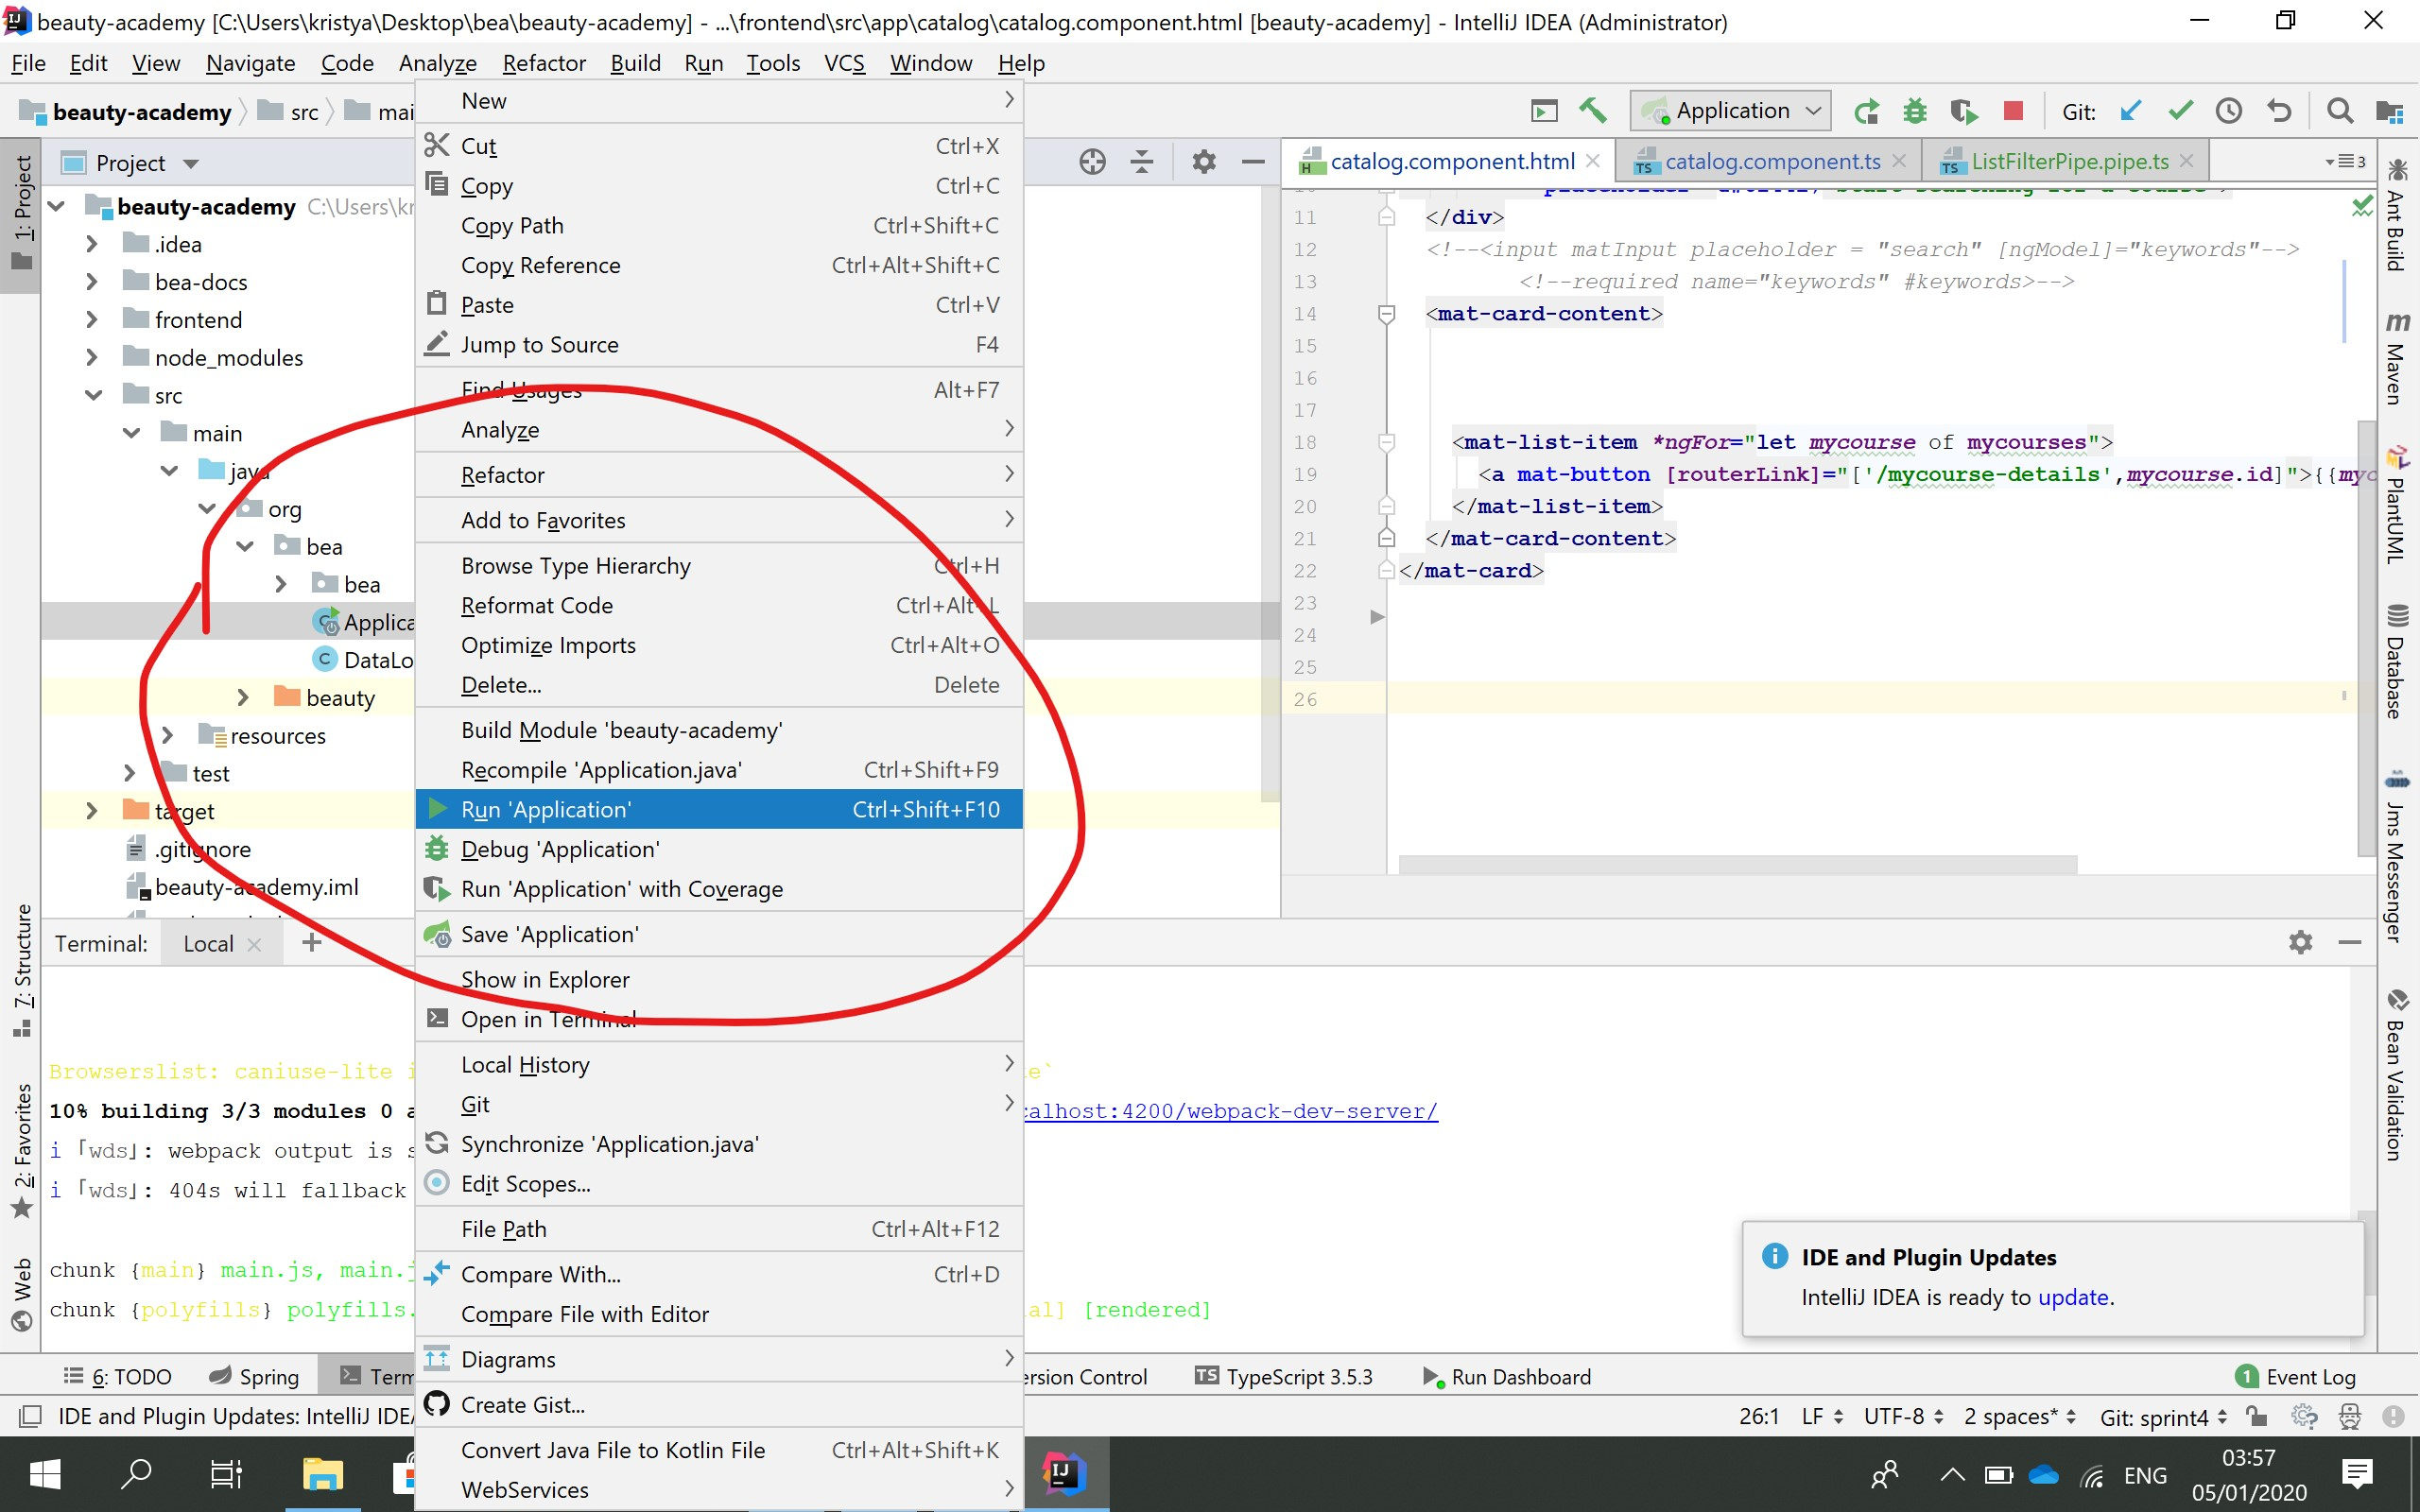
\includegraphics[width=150mm]{run_backend.JPG}
\caption{This figure shows how to run backend of this project}
\label{blabla}
\end{figure}

\begin{figure}[H]
\centering
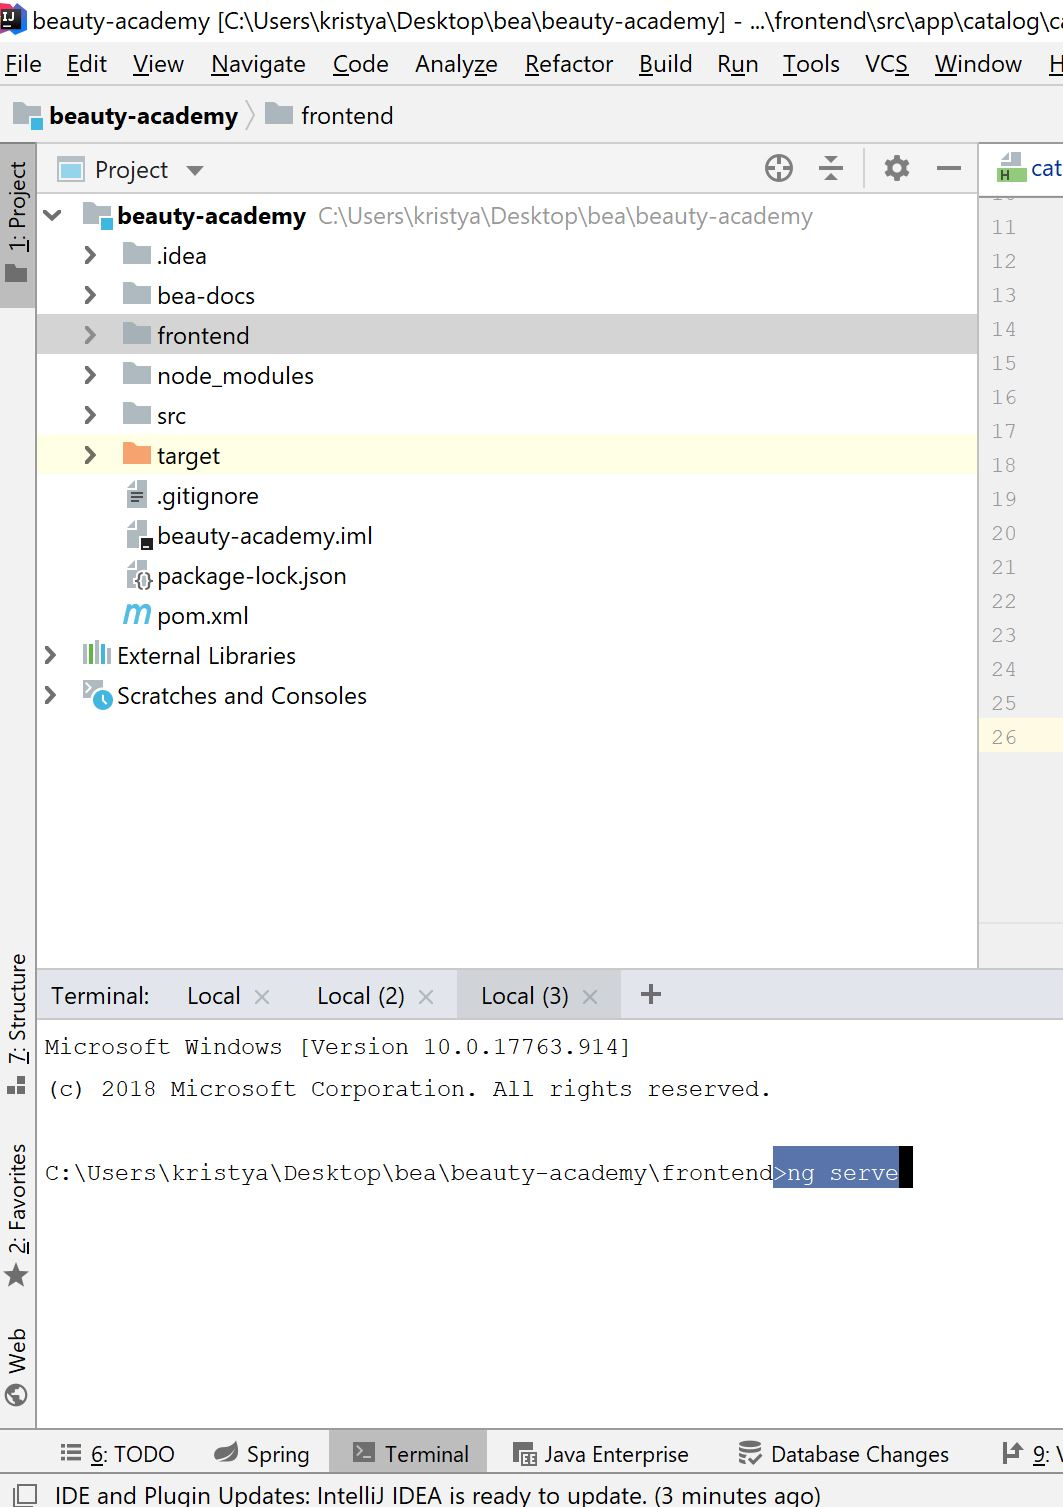
\includegraphics[width=150mm]{run_frontend.JPG}
\caption{This figure shows how to run frontend of this project}
\label{blabla}
\end{figure}

These two figures show how to run this project. First, you have to run backend and then frontend. After this, you have to open the browser on localhost:4200.
\subsection{Integration and System testing}
For testing  this application I have used different tests:\\
• JUNIT I have used as the main testing tool that automates the testing.\\ process.\\
• Checklist to check if we have all functions we need in UI.\\
• Postman to test crud operation in controller\\
• Database Testing. Database is one critical component of this application. Testing actives include:\\
 - Test of any errors while executing code\\
 - Data Integrity is maintained while creating, updating or deleting data in database.\\
 - Test data retrieved from the database is shown accurately in our web application.\\
• Compatibility testing.\\
 - I have used compatibility tests to ensure that our application displays correctly across different devices. This include -\\
 - Browser Compatibility Test: Here we have checked how our application is displayed in different browsers.\\
   The rendering of web elements like buttons, text fields etc. changes with change in Operating System.\\
• Security testing: \\
   Test unauthorized access to secure pages should not be permitted.\\
• Usability testing:\\
  -  Usability test with a small group of students. I have made several scenarios and we have checked how smart our UI logic, and w if there are all necessary tools to use our application.\\



\section{Conclusion and future work}
   \subsubsection{Summary}


After a deep research, I found that there is a lot of information concerning the topic of developing an E-learning management system. To develop even a part of this system is not only a difficult task but also requires a lot of knowledge in software and database design and some programming languages and frameworks like Spring Boot and Angular. \\
I can say that I have achieved my plan, but not completely. I have created the necessary database based on system analysis and implementation. I  have made the system that works, the connection with database, connection between frontend and backend. All concept classes are implemented, so i have good basis to make next implementation of future features.  And I have realised the features like \\
-login\\
-registration\\
-display of course information\\
-managing course information\\
-managing user information \\
The features as course subscription and exam registration are achieved partially .\\
\\ For this document I have used material from course Software Engineering and Design \cite{sed}, Spring Applications course \cite{sf} and tutorials from 'spring.io' \cite{spring-tut} and several tutorials from youtube.\\
To summarise everything I want to say I'm satisfied. It was big work ,very interesting and very different : from analysing to implementation and testing.

 

\subsubsection{Interpretation }

The first thing I want to underline here that the project management has to be done better as I've done this time. I have made big Objective for this project without research how much time I need to improve it.\\
At first, I had to spend more time on analysis what it is really possible to do in this time. For this project, I wanted to use the last technologies. To make it modern and user-friendly. So I had to calculate more time because one of the technologies was new for me. \\
This project I have made from null to the actual state, so it was very important the software engineering steps to do well, using enough time.\\
In the other hand making big Objective, I have achieved also gut results. The biggest part of the project is done.

The conclusion I have made, that to start a project from null I have to calculate much more time as when I have already a concrete assignment.
 

\subsubsection{Outlook}

In this project, I have made an application based on monolith architecture. \\
The goal of future work is instead of continuing to build a large application, is to build a number of smaller microservices. Microservices architecture involves a number of small, well-designed microservices, that exchange messages among themselves.\\
Apart from the better scaling, microservices offer faster development cycles, dynamic scaling depending on load and improved failover behaviour.\\






%% print the bibliography and add the section to the table of content

\printbibliography[heading=bibintoc]

\pagebreak

\section{Project planning}
\subsection{Meetings calendar}

\begin{figure}[H]
\centering
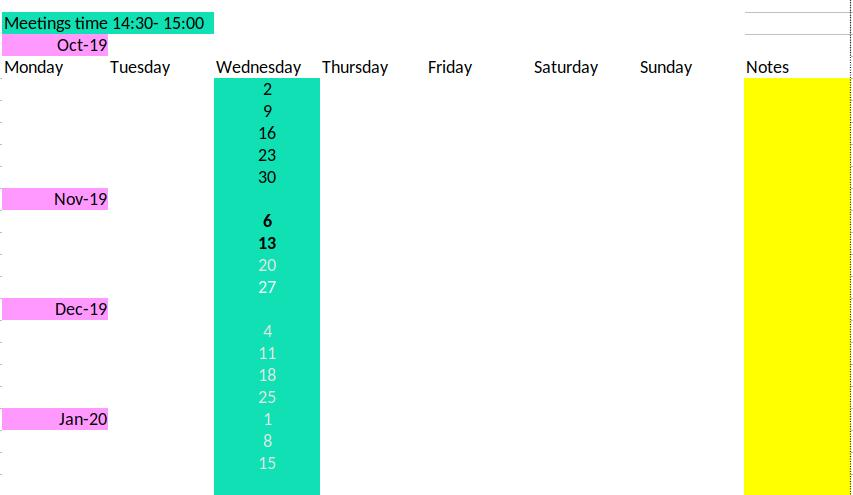
\includegraphics[width = 130mm]{agenda.jpg}
\caption{Meetings calendar}
\label{calendar}
\end{figure}


\subsection{Spring Backlog}


\begin{table}[H]

\begin{center}
\begin{tabular}{| p{2.5cm}| p{4cm} | p{5cm} |p{2.5cm} | p{4cm}|}
   Sprint Backlog of Sprint 1\\ \hline
    
%        \toprule

          \textbf{id}  &  \textbf{Story name} &  \textbf{Story description} &  \textbf{Priority}  & \textbf{Status}\\ \hline
%        \midrule
         0 & Domain model & Domain model & High & done \\ \hline
        1 & Documentation  & Initial structure of main document & High & done \\ \hline
        
           2 &  User stories  & Write some user stories  & High & done. \\ \hline
           3 &  Vision &  Start vision of project & High  & done. \\ \hline
            4 & Infrastructure & Set up infrastructure- Gitlab & done & . \\ \hline
             5 &  User stories & Define more user stories and enter them to the main document. & High & done. \\ \hline
              6 & User stories & Extend user stories with "success" and "failure" & Medium & partial done. \\ \hline
               7 & Infrastructure & Sprint Backlog. Make a document with sprint planning. Divide work in 14 weeks .  & High &  done. \\ \hline
                8 & Documentation & Extend documentation with explanation about Angular and Spring. "What is it Spring, Angular …." & High & done. \\ \hline
                9 & Documentation & Make clear vision document and put it to the main document & High & done . \\ \hline
                  \end{tabular}
    \end{center}
    \caption{Sprint Backlog}
    \label{tab:typo}
\end{table}

\begin{table}[H]

\begin{center}
\begin{tabular}{| p{2.5cm}| p{4cm} | p{5cm} |p{2.5cm} | p{4cm}|}
   Sprint Backlog of Sprint 2\\ \hline
    
%        \toprule

          \textbf{id}  &  \textbf{Story name} &  \textbf{Story description} &  \textbf{Priority}  & \textbf{Status}\\ \hline
               
                
                  10 & Postgres SQL & Add postgres SQL to the project, make connection & High & done. \\ \hline
                    11& UML diagrams & System sequence diagram for login & High & done . \\ \hline
                    12 &  User stories &  Implement login & High & done. \\ \hline
                     13 &  &  &  & . \\ \hline
                       &  &  &  & . \\ \hline
                        &  &  &  & . \\ \hline
         \end{tabular}
    \end{center}
    \caption{Sprint Backlog}
    \label{tab:typo}
\end{table}     

\begin{table}[H]

\begin{center}
\begin{tabular}{| p{2.5cm}| p{4cm} | p{5cm} |p{2.5cm} | p{4cm}|}
   Sprint Backlog of Sprint 3\\ \hline
    
%        \toprule

          \textbf{id}  &  \textbf{Story name} &  \textbf{Story description} &  \textbf{Priority}  & \textbf{Status}\\ \hline            
                    
                 
                    15 & UML diagrams & ssd for registration  & High & .  done\\ \hline
                      16 & User stories & Registration & Hight &  done \\ \hline
                       17 & Front end & Start with frontend & High &   done \\ \hline
                        18 & Documentation & word-->latex & low & . done\\ \hline
                         19 & User stories & Add email confirmation to the registration & Medium & almost done. \\ \hline
                          20 & User stories & Domain classes & High & . done\\ \hline
                           21 & User stories & Repositories and Service classes & High & .done \\ \hline
                            22 & User stories & Add ssd for new feature  & High & . done\\ \hline
                            23 & User stories &  Add Controller for new feature & High & . done\\ \hline
          24 & Front end  & Continue with Angular front end  & High & . done\\ \hline
          
            \end{tabular}
    \end{center}
    \caption{Sprint Backlog}
    \label{tab:typo}
\end{table}
          
          \begin{table}[H]
%    \centering
%    \begin{tabular}{c@{\qquad}lllll}
\begin{center}
\begin{tabular}{| p{2.5cm}| p{4cm} | p{5cm} |p{2.5cm} | p{4cm}|}
   Sprint Backlog of Sprint 4\\ \hline
    
%        \toprule

          \textbf{id}  &  \textbf{Story name} &  \textbf{Story description} &  \textbf{Priority}  & \textbf{Status}\\ \hline
	
%	Spring Backlog of Sprint 4\\
	 25  & User stories & Connect crud methods to the frontend & High & . done\\ \hline
	  26  & Frontend & Make new components for catalogue details  & High & . done\\ \hline
	    27 & Report & Make more sd diagrams & High & . done\\ \hline
	     28  & Report  & Add Summary, Abstract and another parts to document & High & . done\\ \hline
	    29   & Report & Check of grammar  & High & done. \\ \hline
	        &  &  &  & . \\ \hline
	         &  &  &  & . \\ \hline
	         &  &  &  & . \\ \hline
	           &  &  &  & . \\ \hline
	            &  &  &  & . \\ \hline
	             &  &  &  & . \\ \hline
	              &  &  &  & . \\ \hline
	               &  &  &  & . \\ \hline
	
	 
        
    \end{tabular}
    \end{center}
    \caption{Sprint Backlog}
    \label{tab:typo}
\end{table}

   

   
    
   
  

\subsubsection{Protocol}
\textbf{\textit{Frequency: (weekly) \\
Meeting length: (35-45 minutes)}}\\

Agenda

\begin{itemize}
  	\item Demo and Discuss Deliverable(Demo)
  	\item Planning next Goals(Plan)
  	\item Lessons learned (Lessons)
  	\item Date, time of the next meeting(next meeting)
 \end{itemize} 	


\textbf{\textit{Report from 09.10.19}}\\
Plan\\
Next goals are: 
\begin{itemize}


	\item Introduction of a Vision make clear. Write about an application I want to build. I have to write a Vision that can make a good picture about the functionality of this application.
	\item	Change the problem statement: 
	\item	Join 2 Systems in 1 . Rename system in functions. And write that these functions just a part of this system we want to build. 
	\item	Write concrete user stories to these functions, group the stories according the function.
	\item	Analyze domain model, put attributes to each conceptual class, make description for each association. Rebuild domain model according of new clear representation of necessary functions of the system.
	\item	Sequence diagram of first function we want to implement (probably log in)
	\item	Try to make class-diagram.
	\item	Implement of log in function.
	\item	Write a protocol in the main doc.
\end{itemize}	
Lessons learned\\
To documentation plays decisive role in Software Engineering Project. The first analysing phase have to be done well to make a good start for design and implementation of the IT Product.
Next Meeting: 16.10.19, 14:30\\




\textbf{\textit{Report from 16.10.19}}\\
Plan:\\
The next goals are:\\
\begin{itemize}


	\item	A domain model – last version. +
	\item	Vision complete. +
	\item	Put spring plan in the main document (Time planning is the first preference).
	\item	After completing 3d point, merge sprint1 and make a del1.
	\item	Start with Design part: 1st we start with design for login feature.+
	\item	SSD for login +
	\item	Write good document for Spring Boot and Angular. Describe the most successful aspects,that has spring boot , angular. Describe why we have chosen it for this project. Describe how can be implement login with spring boot.    +
	\item	Make a Product Backlog( list of user stories) and divide to 4 sprints. +
	\item	Point 1 and 2 have highest priority. Just when these 2 points successfully completed I will continue my  to-dos.  +
	\item	Change the style of document, make headers numerable, and the style more readable.  +
 \end{itemize}
Lesson Learned\\
With this practical work I become always clearer the main principles of building software.\\

Next meeting:		23.10.19, 14:30\\



\textbf{\textit{Report from 23.10.19}}\\

Plan:
\begin{itemize}


 
	\item	Make Vision clear( Describe how people will use this application. Describe what is it exactly the course(content, PDF, Unterricht) The vision needs to be loner ,about 1 A4 page.
Vision-Solution belongs to Vision, here I have to write what we will produce.
	\item	Domain model. Change word entity to concept by description.
Add two concepts: subscription with a Date attribute .
Add to exam concept boolean , that will show the difference between final and intermediate exam.
	\item	Change product backlog (failure and success) 
	\item	Make ssd for login with all needed classes( show exactly what’s happened in system ). 
	\item	Implement login function, test it. Have to be able to make a demo.
	\item	After making all 5 points and if I’ll have more time make ssd for other features.
	\end{itemize}
Lesson learned: \\
More experience about software engineering diagrams\\
Next meeting: 30.10.19, 14:30\\


\textbf{\textit{Report from 30.10.19}}\\
Plan:\\
\begin{itemize}


	\item	Start frontend with Angular. Make frontend for login and registration.
	\end{itemize}
Lesson learned:\\

Next meeting: 06.11.19, 14:30\\



\textbf{\textit{Report from 06.11.19}}\\
Plan:\\
\begin{itemize}


	\item	Documentation
	\item	Most important thing in a documentation is to write it so that the reader can easily understand the main scope of project, how it will be realised, etc.  
	\item	Angular and spring . Make description of angular and spring , reader have to understand for what we use exactly this frameworks. (have to notice in bibliography everything I use from other authors)
	\item	Make a build of architecture of angular and spring( probably layers build)
	\item	Vision more
	\item	User-stories
	\item	Agile and scrum -\/
	\item	Make registration with via email address. (read about registration via facebook, ect if I have more time)
	\item	 Start to learn about micro services. Try to add first documentation about it. 
\end{itemize}
Lesson learned:\\
Today I’ve learned that I have to plan my work better, means that first I have to realise the most difficult and most important tasks, and then make tasks less difficult. \\
 
Next meeting: 13.11.19, 14:30\\





\textbf{\textit{Report from 13.11.19}}\\

Plan:\\
\begin{itemize}
	\item	Documentation: 
Describe:\\
        What is it monolith architecture, what is different from monolith and micro services?\\
       What is restful? (in layer diagram)\\
	\item	Code \\
Make registration via email. Start other features. This step I have to do just when I have finished the documentation.
For next time be able to make a demo of what we have.
\end{itemize}

Lesson learned:\\
Be able to define clear the features I want to realise in this project.\\
Next meeting: {27.11.19, 14:30} \\




\textbf{\textit{Report from 27.11.19}}
Plan:\\
\begin{itemize}
	\item	Add version to each technology .

	\item	Describe in report how to use this application(how to compile(localhost: ...).
	\item Make good description of layer bild.

\end{itemize}

Lesson learned:\\ Learned more about writing professional documents. New tips about system sequence diagram.

Next meeting: {11.12.19, 14:30}


\textbf{\textit{Report from 11.12.19, }}
Plan:\\
\begin{itemize}
	\item	 Continue making report 
	
	\item	Continue with implementation

\end{itemize}

Lesson learned:\\

Next meeting: {08.01.20, 14:30}


\textbf{\textit{Report from 08.01.20 }}
Plan:\\
\begin{itemize}
	\item	 Prepare presentation 

	\item	 Complete all work until deadline. Merge the print 4 to the master. Make separated doc folder that will contain final report in pdf only. 

\end{itemize}

Lesson learned:\\ Learned some presentation staffs

Next meeting: \\ {presentation}


\end{document}


